\section{Markov Chain Monte Carlo Methods} \label{MCMC_SECT}
\subsection{Bayesian Techniques} \label{Bayesian_Techniques}
Bayesian inference is a powerful tool in parameter estimation for biological systems that begins with previously known information and updates a system using new, incoming data \cite{bayesian_param_inf}.  In particular, Bayesian inference techniques have been used to parameterize a variety of biological models and systems, \cite{bayesian_param_inf_ex1}, \cite{bayesian_param_inf_ex2}. In the following sections, we outline the basic mathematical concepts behind the Bayesian inference technique Markov Chain Monte Carlo (MCMC) method, introduce two specific implementations of MCMC methods, and parameterize two different biological nonlinear ODE systems.
\subsubsection{Bayesian Parameter Estimation}
Bayesian parameter estimation is a process of inferring a posterior probability density function (PDF) over a model's possible parameters given data, $D$, for some model, $M$ \cite{astrostats}. This PDF can be evaluated for a set of parameters, giving individual probabilities. Parameters of a system are treated as random variables and realized as $\theta = [p_1, p_2,...,p_n]$, where $p_i$ is a parameter of a modeling system. They follow distributions that incorporate both \emph{a priori} knowledge such as mathematical models or theory, about their values, as well as information obtained from data collection. When estimating a system's parameters, $\theta$, a variety of Bayesian techniques can serve to find a posterior density, the post-parameterization distribution of parameter values based on sampled data and a given model \cite{bayesprior}. This technique relies on Bayes' Theorem which is defined as follows:
\begin{equation} \label{eq:1mcmc}
P(\theta | D, M) = \frac{P(D|\theta, M)P(\theta|M)}{P(D|M)}
\end{equation}
where $\theta$ denotes a set of parameters. $P(D|\theta, M)$ is referred to as the \emph{likelihood} and denotes the probability of the data given the current parameters and model \cite{astrostats}. $P(\theta|M)$, or the \emph{prior}, gives the probability of a set of parameters for a given model, before the data can inform the system \cite{astrostats}. Finally, the denominator $P(D|M)$ is known as the \emph{evidence} \cite{astrostats}. The evidence (also called the normalization constant of the posterior probability) does not depend on $\theta$. In mathematical terms, because our posterior, $P(\theta|D,M)$ is a \textit{density function}, we need the right hand side of \textbf{Eq. \ref{eq:1mcmc}} to integrate to 1 (and avoid a situation of dividing by 0) \cite{bayesprior}, without the normalization constant, this is not possible. However, it is often difficult to calculate $P(D|M)$ (as the integral may not be closed-form) and many mathematicians choose to work with a variation of Bayes' Theorem:
\begin{equation} \label{eq:2mcmc}
P(\theta|D,M) \propto P(D|\theta,M)P(\theta|M)
\end{equation}
as it is possible to compute the priors and likelihoods. We work initially with \textbf{Eq. \ref{eq:1mcmc}} in this tutorial, but 
through derivations shown in Section \ref{The_Likelihood_Function}, we arrive at Eq. \ref{eq:2mcmc}. Thus the quality of posterior estimation relies heavily on choices of the likelihood and prior which are informed by \textit{a priori} knowledge.
\paragraph{The Curse of Dimensionality}
Many models have a significant number of parameters which leads to a high-dimensional parameter space, and thus a high dimensional posterior PDF. The best-fit set of of parameters for the model would be located at the peak of this multi-dimensional PDF, as these are, by definition the parameters located at the highest probability of the overall modeling system. 
\par Due to the unknown shape of the PDF, this maximum likelihood cannot be found analytically. Additionally, searching for it directly (discrete calculations for example) poses a challenge. While sufficiently sampling a one-dimensional PDF might require $N$ samples, sufficiently sampling a two-dimensional PDF requires building a grid of $N^{2}$ samples, and a $j$-dimensional PDF consequently requires a hypercube of $N^{j}$ samples. This exponential increase is known as the \emph{curse of dimensionality} \cite{astrostats}. Evaluating the posterior PDF for $N^{j}$ samples is computationally infeasible. Moreover, the probability of the majority of the these coordinates is very small adding to the computational difficulty. To overcome the curse of dimensionality, we instead look to \emph{sample} the posterior PDF directly. In effect, these samples simulate the distribution itself and feasible predicted values of parameters can be extracted from the simulation. One class of methods for such sampling is known as Markov Chain Monte Carlo methods, or MCMC methods. We will explore two MCMC algorithms and parameterize both the Lotka-Volterra and Type 1 Diabetes mathematical models. 

\subsection{Markov Chain Monte Carlo Sampling} \label{Markov_Chain_Monte_Carlo_Sampling}
Markov Chain Monte Carlo methods are used to describe posterior distributions when there is incomplete knowledge of the distribution's properties (such as its mean or variance) \cite{MLEvsBayes_powerpoint}. 
\par The idea driving MCMC is that of \textbf{Monte Carlo} methods. We are working in probabilities (via Bayes' Theorem), thus we rely on the probabilistic Monte Carlo method in which we observe quantities chosen to simulate the physical or biological processes of our model and infer a solution from their behavior \cite{montecarlo}. In the context of ODE system parameterization, we draw samples of parameters from an arbitrary probability density using random numbers drawn from a simpler distribution \cite{astrostats} and infer posterior probabilities. MCMC uses a \textbf{Markov Chain} to perform \emph{rejection sampling} - that is, given a proposal distribution (a distribution of parameter values that we draw candidates from), we draw samples and penalize with an acceptance criteria (a ratio). Briefly, a Markov chain is a process in which we move among a set of elements $X$ according to a specified probability. Beginning at element $x_1 \in X$ we move to $x_2 \in X$ according to a probability distribution $P(x_1, *)$ which depends only on $x_1$ \cite{markovchains}. We use an asterisk to signify a multitude of possible probabilistic rules that could be applied that depend on the specifics of a model. For example, in a very simple system, let us say that we have a sequence of values $[0,1,...10]$. We might start at a value 0 and move with probability $\frac{1}{3}$ to an even value, move with probability $\frac{1}{3}$ to an odd value, and stay at 0 with probability $\frac{1}{3}$. The Markov ``chain" refers to the order and values of elements in $X$ that we have visited (or collected).
The Markovian aspect of this algorithm establishes a random walk over the parameter space such that we can preferentially sample regions of high probability. Furthermore, since each `step' along this walk is only dependent on the previous, we classify the MCMC as a first-order Markovian process \cite{firstorderMarkovian}. 

\par The umbrella of MCMC methods is broad, but here we introduce implementations of the simplest algorithm, Metropolis MCMC, as well as a method derived from Metropolis, delayed rejection adaptive Metropolis (DRAM) MCMC. We find that looking at these two methods of sampling gives the reader a good idea of the range of capabilities that MCMC can provide for parameterization. Metropolis MCMC provides the most basic search in parameter space and is likely to find local probabilistic maxima (rather than global maxima). That is, due to the algorithm's search method, Metropolis MCMC will tend to settle in an area of parameter space with high probability according to the model and rarely move into areas of lower probability. This is detailed in Section \ref{Metropolis_MCMC}. DRAM on the hand, is more likely to find global probabilistic maxima as the algorithm is able to search and sample lower probability parameter space.

\subsubsection{Defining Bayes' Theorem} 
Bayes' Theorem is the underlying framework in the MCMC algorithm of accepting and rejecting samples. In this section we further specify elements of Bayes' Theorem in terms of a mathematical model and its parameters following a tutorial in \cite{astrostats}. We introduce two new concepts: the proposal distribution from which we draw parameter samples and the acceptance criteria which we use to accept and reject candidates.
\paragraph{The Prior Distribution} \label{section:ThePriorDistribution} The \emph{prior function} is the uncertainty that we have about a specific set of parameters \emph{before} we observe any data and informs us how likely we are to have sampled that set of parameters \cite{astrostats}. We can specify the prior distribution based on \textit{a priori} knowledge about our biological system \cite{bayesprior}. For example, if we know from previous experimentation the range of variation that we expect a parameter to exhibit, we can constrain the parameter candidates that we draw accordingly. However, when we know nothing about our parameter values, we initialize an uninformative prior distribution - a uniform distribution \cite{astrostats}:
\begin{center} \label{eq:3mcmc}
\begin{align}
  P(\theta|M) = \left\{ \begin{array}{cc} 
                \frac{1}{b-a} & \hspace{5mm} a \leq \theta \leq b \\
                0 & \hspace{5mm} otherwise \\
                \end{array} \right.
\end{align}
\end{center}
It is important to note that we must know enough about the parameters of the system in order to make a decision about the bounds of the uniform distribution. When implementing a prior function, we specify the range of the distribution such that the values of $\theta$ will always be constrained between the bounds. For example, in a biological system we could say that it is biologically infeasible for a particular parameter value to be negative. In effect, we do not want our prior function to be 0 because in computing the acceptance ratio (discussed in \ref{The_Acceptance_Criteria}), we will encounter a situation of dividing by 0. Consequently, the prior distribution becomes
\begin{equation} \label{eq:4mcmc}
P(\theta|M) = \frac{1}{b-a}
\end{equation}
That is for any values of $\theta$ our prior distribution will be never be 0. It is important to point out with this definition, we have specified the same uniform interval, $[a, b]$, for all parameter sets. Now what does this mean in the context of parameterization and why would we choose to do this? If we truly have no \emph{a priori} information about our model and its parameters, then we do not want to implement any bias when accepting and rejecting samples. In other words, we want each sample to be equally likely (in terms of being informed by the prior) and the uniform prior achieves this for us. 
\paragraph{The Likelihood Function} \label{The_Likelihood_Function} The \emph{likelihood function} represents the relationships between independent evaluations of a model (given specified parameters) and it informs us \emph{how} to accept samples of parameters from the specified proposal distribution. In a biological model, we would assume that there exists some amount of error, or noise, within the model itself. If we have $D = \{x_1,...,x_n; y_1,...,y_n\}$ with $n$ data points, then our model $M$ predicts values of $y$ to be
\begin{align} \label{eq:5mcmc}
y_1 = f(x_1) + \epsilon_1 \cdots y_n = f(x_n) + \epsilon_n
\end{align}
where $f(x_i)$ is the evaluation of the ODE system and $\epsilon_i$ is our system noise \cite{astrostats}. The most general assumption we can make is that the noise is an independent and identically distributed (every random variable has the same distribution and each is independent of the others) Gaussian distribution with a mean of 0 and a standard deviation $\sigma$. 
\par The distribution of the likelihood informs us how different evaluations of the model are distributed given varying parameter values \cite{smithCh8}. Thus, when we accept sampled parameter values, we will do so according to the likelihood function's distribution. Often, the likelihood is given as a normal distribution
\begin{equation} \label{eq:6mcmc}
    P(D|\theta, M) = \frac{1}{\sigma \sqrt{2\pi}} e^{-\frac{SS_{\theta}}{{2\sigma^2}}}
\end{equation}
where $SS_{\theta} = \sum_{i=1}^{n}[y_i - f_i(\theta)]^2$ is the sum of squares error between the predicted model and the original data and $\sigma$ refers to the standard deviation of the noise \cite{smithCh8} \cite{astrostats}.
\par It is important to note that $\sigma$ is often unknown. We may know that our system produces some noise, but we are not able to quantify it via a specific standard deviation. In this case, we can simply use an estimate for $\sigma$, denoted as $s$. There are a variety of ways to estimate $s$, however in practice, we use the following estimation
\begin{equation} \label{eq:7mcmc}
s^2 = \frac{SS_{\theta}}{n-p}
\end{equation}
where $n$ is the total number of data points, $p$ is the number of parameters and $SS_{\theta}$ is as defined above \cite{smithCh8}.
\paragraph{The Posterior Distribution} The \emph{posterior distribution} is the accumulation of samples in the chain that are accepted and to which a distribution can be fitted. Not only can we extract the PDF of a set of parameters, we can extract individual parameter PDFs \cite{astrostats}.
\paragraph{The Proposal Distribution} We now must introduce a new element that is not a part of Bayes' Theorem: the proposal distribution. This is the distribution from which we draw the values of our samples. If we have \textit{a priori} knowledge about our parameter space, we can specify our own distribution, but when no knowledge is available, a normal distribution is often assumed \cite{astrostats} \cite{bayesprior}. For certain MCMC algorithms, like the Metropolis MCMC, the proposal distribution must be symmetrical \cite{smithCh8}. A proposal distribution $J$ is considered symmetrical if $J(\theta^{*}|\theta^{k-1}) = J(\theta^{k-1}|\theta^{*})$, where $\theta^*$ is the proposed sample and $\theta^{k-1}$ is the current sample \cite{smithCh8}. In symmetric sampling, the order of selecting parameters does not matter; that is, the probability of moving from sample $a$ to sample $b$ is the same as moving from $b$ to $a$.
\par In order to get the best parameterization of our model, we want to establish a proposal distribution from which we believe we will be able to sample the best values for our model. In practice, it is common to initialize a multivariate Gaussian distribution \cite{astrostats} \cite{mcmcstatlib}. We can implement a covariance matrix to represent this proposal distribution. The coefficients of this matrix will represent the effect that perturbations of varying parameter values may have on the system \cite{sensitivity_matrices1}. In our Gaussian proposal scenario, we define the proposal 
\begin{equation} \label{eq:8mcmc}
V = J(\theta^*|\theta{k-1})
\end{equation}
where $J$ is defined as a Jacobian output matrix \cite{sensitivity_matrices1} \cite{smithCh8}. The proposal is distributed as $N(\theta^{k-1}, V_{cov})$ where $V_{cov}$ is the covariance matrix for $\theta$ \cite{smithCh8}. (Note that $V_{cov}$ must be positive definite.) In the \texttt{mcmcstat} library function \texttt{mcmcrun}, this covariance matrix is computed internally \cite{mcmcstatlib}.
\par One way to construct $V$ by hand is to use a sensitivity matrix. Briefly, this matrix is calculated by computing the Jacobian matrix of the derivatives of the parameters and the model. For a more in-depth calculation of $V$ we refer the reader to \cite{smithCh8} and \cite{sensitivity_matrices1}.
\paragraph{The Acceptance Criteria} \label{The_Acceptance_Criteria} As we pointed out before, the acceptance criteria is the element of MCMC sampling that allows the algorithm to accept and reject proposed samples in the Markov chain. We want to discriminate between samples of parameters based on their probabilities, only accepting the best (the most likely according to our likelihood, prior, and proposal functions) sets. To do this, we accept parameter sets according to a ratio, $\alpha$, which is a direct application of Bayes' Theorem \cite{astrostats}. While $\alpha$ may differ slightly according to the specific MCMC algorithm begin implemented, a basic ratio compares the posteriors of a proposed set of parameters ($\theta^*$) with the last accepted set of parameters ($\theta^{k-1}$) as follows:
\begin{equation} \label{eq:9mcmc}
\alpha = min(1, \frac{P(\theta^*|D, M)}{P(\theta^{k-1}|D,M)}) = min(1, \frac{\frac{P(D|\theta^*, M)P(\theta^*|M)}{P(D|M)}}{\frac{P(D|\theta^{k-1}, M)P(\theta^{k-1}|M)}{P(D|M)}}) = min(1, \frac{P(D|\theta^*, M)P(\theta^*|M)}{P(D|\theta^{k-1}, M)P(\theta^{k-1}|M)})
\end{equation}
Notice that the \emph{evidence} term of Bayes' Theorem (the denominator) cancels out. Intuitively, this cancellation makes sense because we are only interested in comparing the impact of different parameter sets on the model, but the evidence does not depend on the parameters at all. If 
\begin{equation} \label{eq:10mcmc}
P(D|\theta^*, M)P(\theta^*|M) \geq P(D|\theta^{k-1}, M)P(\theta^{k-1}|M)
\end{equation}
we accept $\theta^*$ with a probability of 1. If this is not the case, we still want to accept $\theta^*$ with some probability, the ratio between products of likelihoods and priors \cite{astrostats}. We never want to perform an immediate rejection of any parameter set because we assume that we will find a majority of our ``best" parameter values given the prior and likelihood functions that we have chosen. Thus, while a candidate may not be the best parameter set according to $\alpha$, it can still inform our posterior distribution. So, we want some probability of accepting any sampled parameter set. In addition, if we outright reject any candidate that does not meet the acceptance criterion, we run the risk of getting stuck in a very small range of values to sample from since our next parameter candidate depends directly on the previously sampled (and accepted) parameter set due to the Markovian process of the algorithm.
\par To get a better understanding of how $\alpha$ is constructed, let's use our Gaussian likelihood and uniform prior on the interval $[a, b]$. The acceptance criterion becomes
\begin{equation} \label{eq:11mcmc}
\alpha = min(1, \frac{P(D|\theta^*, M)(\frac{1}{b-a})}{P(D|\theta^{k-1},M)(\frac{1}{b-a})}) = min(1, \frac{\frac{1}{\sigma \sqrt{2\pi}} \exp^{\frac{SS_{\theta^*}}{{2\sigma^2}}}}{\frac{1}{\sigma \sqrt{2\pi}} \exp^{\frac{SS_{\theta^{k-1}}}{{2\sigma^2}}}})
\end{equation}
which simplifies to
\begin{equation} \label{eq:12mcmc}
    \alpha = min(1, exp^{-[-SS_{\theta^*} - SS_{\theta^{k-1}}]/2\sigma^2}) \cite{mcmcstatlib}
\end{equation}
\paragraph{Overview} So how does sampling create a usable posterior distribution? Figure 1 illustrates the MCMC process.
\begin{figure}[H]
    \centering
    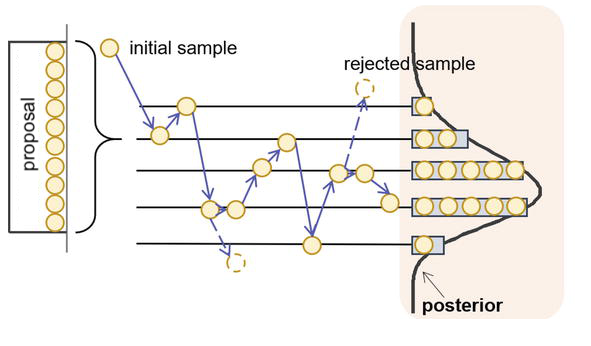
\includegraphics[width=15cm]{MCMC_figs/mcmc_procedure.png}
    \caption{Markov chain Monte Carlo sampling using random walk. Image adapted from \cite{mcmcFig} Figure 3.}
\end{figure}
We start with a general pool of potential parameter values - our proposal distribution. As we iterate through the chain, accepting and rejecting a samples - using the acceptance criterion, eventually we can fit our accepted samples to a distribution, the posterior distribution.
\subsection{Metropolis MCMC} \label{Metropolis_MCMC}
The single-chain Metropolis MCMC algorithm is one of the most basic and widely implemented MCMC methods. The simple acceptance-rejection method of sampling means that the Metropolis MCMC method tends to find local probabilistic maxima as once it has determined a high probability range of values within the parameter, it is unlikely to explore further away from that area. The Metropolis algorithm is a special case of another common MCMC algorithm, the Metropolis-Hastings algorithm \cite{metropolis1953}. The Metropolis algorithm requires a symmetric proposal distribution, whereas Metropolis-Hastings does not \cite{smithCh8}. Below, we outline the algorithm for the the Metropolis MCMC method.
\begin{tcolorbox} \label{alg:met}
\textbf{\underline{Metropolis MCMC Algorithm (with an uninformative prior)}} 
\begin{enumerate}
    \item Set number of samples to take, $N$ and determine a burn-in period, $k_b$
    \item \label{step:2met} Determine an initial parameter guess, $\theta^0 = argmin_\theta \sum_{i=1}^{n}[M_i - f_i(\theta)]^2]$

    \item Set $SS_{\theta^0} = \sum_{i = 1}^{n}[y_i - f_i(\theta^0)]^2$ (for initial likelihood, see \ref{The_Likelihood_Function})
    \item Compute an initial error variance estimate $s_0^2 = \frac{SS_{\theta^0}}{n-p}$ ($n = $ number of data points, $p = $ number of parameters)
    \item Construct proposal covariance matrix $V$
    \item \label{step:6met}For each iteration of the chain, $k = 1,...,N$ 
    \begin{enumerate}
        \item Sample $z \sim N(0,I_p)$ 
        \item Construct candidate $\theta^* = \theta^{k-1}+ Vz$
        \item Compute $SS_{\theta^*} = \sum_{i = 1}^{n}[y_i - f_i(\theta^*)]^2$ (for likelihood)
        \item Compute acceptance criterion
            \begin{center}
                $\alpha(\theta^* | \theta^{k-1}) = min(1, \frac{P(\theta^* |D, M)}{P(\theta^{k-1}|D, M})) = min(1, e^{-[SS_{\theta^*}-SS_{\theta^{k-1}}/2s_{k-1}^2]})$
            \end{center}
        \item Accept $\theta^*$ with probability 1 if $\alpha \geq 1$ and accept it with probability $\alpha$ if $\alpha < 1$.
        \begin{itemize}
            \item If $\theta^*$ is accepted
            \begin{center}
                $\theta^k = \theta^*$, $SS_{\theta^k} = SS_{\theta^*}$
            \end{center}
            \item Else
            \begin{center}
                $\theta^k = \theta^{k-1}$, $SS_{\theta^k} = SS_{\theta^{k-1}}$
            \end{center}
        \end{itemize}
        \item If $k > k_b$ collect $\theta^*$ in posterior matrix $P$, else discard.
        \item Update $s_k^2 = \frac{SS_{\theta^k}}{n-p}$
    \end{enumerate}
\end{enumerate}
\emph{Based on Smith (2014) Algorithm 8.5}
\end{tcolorbox}
\par We want to determine a number of samples to take, $N$ so that we can be sure that the resulting accepted parameter values approach the posterior distribution. Since we are sampling a parameter space via random-walk (since $\theta^*$ only relies on $\theta^{k-1}$), we want our algorithm to settle into an area of values that are highly likely to fit our model $M$. Thus, we want the chain to reach \emph{convergence} or a steady state. We can increase the likelihood of convergence occurring by performing \emph{burn-in} iterations ($k_b$) of the chain. That is, we sample according to the Metropolis algorithm, however we must discard the beginning of the chain. This allows the chain to explore the parameter space, determine local maxima, and increases the probability that when we collect samples, they will reflect our desired posterior. The burn-in period is a sliding scale and can be determined mathematically \cite{rafferty1992burnin}, however, in this tutorial we implement a burn-in of  $\sim 10\%$ of the total chain length as this is a common percentage of samples in the literature.
\par Note that in Step \ref{step:2met}, $\theta^0$ is found by minimizing the ODE model and extracting the parameter values. In practice we use the MATLAB \texttt{fmincon} function to do this. It should be noted that initial values of $\theta$ may be found in different ways, for instance if the user may specify values based on previous experimentation or calculation. In Step \ref{step:6met}a, we sample a normal value $z$ such that $z \sim N(0,I_p)$ where $I_p$ is an identity matrix of $p$-by-$p$ (the number of parameters) dimensions. Intuitively, $z$ is the random component of selecting a parameter set and is what makes each $\theta^*$ unique even if multiple $\theta^*$s are found using the same $\theta^{k-1}$. Since our $V \sim N$, $z$ must also be Gaussian. Note that in Step \ref{step:6met}b, we can see the Markovian influence as the candidate parameter is selected based on the previously accepted parameter set.

\subsubsection{Parameterizing Lotka-Volterra} Parameterizing a simple biological model using the Metropolis method is a good way to get familiar with the role of the elements of Bayes' Theorem and MCMC. Here we have parameterized the classic predator-prey model in MATLAB based on a tutorial in R originally intended for parameterizing a small non-linear ODE system \cite{mcmcstatlib}. It is important to note that MATLAB has its own implementation of the Metropolis MCMC method, \texttt{mhsample}. However, using this function requires an initialization routine similar to the one that we outline here. We are using the functions from the MATLAB \texttt{mcmcstat} library \cite{mcmcstatlib} and so we implement the components of the Metropolis MCMC method according to requirements of this algorithm. 
\par We consider 4 parameters in this model: $\theta = \{ \alpha, \: \beta,\: \delta,\: \gamma \}$ (full details of the Lotka-Volterra ODE model can be found in Section \ref{Lotka_Volterra_System}). We begin our parameter estimation by establishing an initial guess for our parameter values and their ranges (see \ref{section:LV_params} for details). As a general guide for creating our parameter ranges, we knew that our parameter values would never be negative. Through experimentation, we found that a good starting place would be to have a range of $\pm$ a reasonable percentage (at maximum 100$\%$) and to constrain the lower end of the range to 0. We settled on using a range of $\pm 10\%$ of our initial parameter values as this seemed to create a sufficient parameter space for sampling. We assume a Gaussian likelihood function in log (base e) form (Step 3). Due to the sum of squares calculation for the likelihood function (see Section \ref{The_Likelihood_Function}) we will be dealing with larger numbers (on the scale of 10e03 to 10e04). Thus, the natural log form is chosen for computational ease as we are able to compute sums rather than products and prevent exponential increase in values. The sum of squares between the model given parameter values and the original data is thus
\begin{equation} \label{eq:13mcmc}
lnP(D|\theta, M) = \sum_{k=1}^{N}lnP(y_k|x_k,\theta,M) = \sum_{k=1}^N SS_\theta^k
\end{equation}
 We also adopt a log-uniform prior with bounds $[0,1]$ (recall Section \ref{section:ThePriorDistribution})
\begin{equation} \label{eq:14mcmc}
lnP(\theta|M) = ln\frac{1}{1-0} = 0
\end{equation}
The proposal distribution is determined for us in the MATLAB function \texttt{mcmcrun} using a covariance matrix (Step 5). The acceptance criteria (Step 6d) according to the \texttt{mcmcstat} library is defined as
\begin{equation} \label{eq:15mcmc}
\alpha = min(1, e^{ \lbrack {-0.5(\frac{\sum (SS_{\theta^*}-SS_{\theta^{k-1}})}{\sigma^2} + prior^*-prior^{k-1})} \rbrack})
\end{equation}
and thus with our assumptions simplifies to 
\begin{equation} \label{eq:16mcmc}
\alpha = min(1, e^{[ {-0.5(\frac{\sum (SS_{\theta^*}-SS_{\theta^{k-1}})}{\sigma^2}]}})
\end{equation}

With all of these assumptions and initializations, we can run the Metropolis MCMC algorithm and produce PDFs for each of our parameters. 
\paragraph{Analyzing the Chain} \label{Analyzing_the_chain_Met}
Let's look at how our algorithm works by first visualizing the chain samples.
\begin{figure}[H]
    \centering
    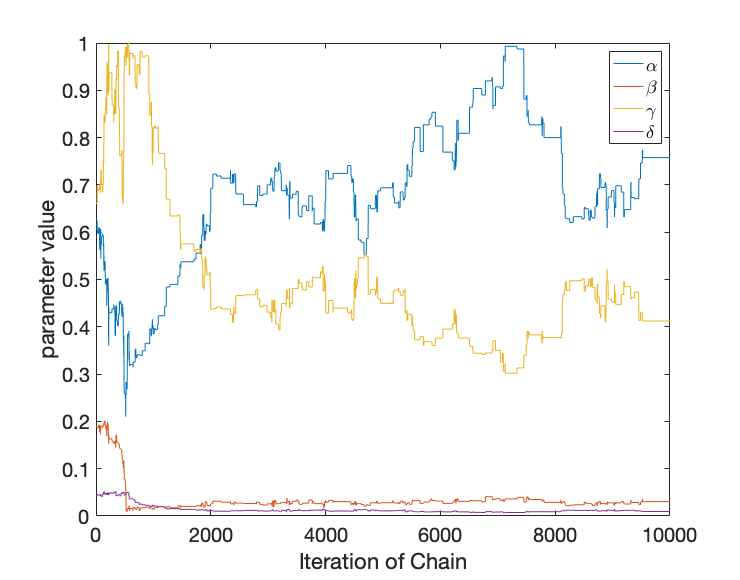
\includegraphics[width=15cm]{MCMC_figs/met_lv_final/final_mh_burninchain.png}
    \caption{Trace plot for the burn-in chain (10,000 samples) for the Metropolis MCMC parameterization of the Lotka-Volterra model. Each line shows the sampled parameter values. This figure illustrates the movement of the Markov chain as it samples parameters with the goal of finding the most likely range of values. As expected, the chain has not completely converged yet.}
    \label{fig:1mcmc}
\end{figure}
In Figure \ref{fig:1mcmc}, we can see the ``movement" of the chain as it looks around the parameter space drawing values. We have implemented and visualized a burn-in period of 10,000 chain samples. In Figure \ref{fig:1mcmc}, it appears that the values of $\alpha$ and $\gamma$ are changing fairly drastically for every sample as evidenced by their more pronounced upward and downward trends. On the other hand, $\beta$ and $\delta$ seem to have less drastic value changes appearing to reach a steady state before 2,000 samples. It is also interesting to note that the trace plots for $\alpha$ and $\gamma$ appear to mirror each other: as $\alpha$ decreases, $\gamma$ increases and vice versa. Recall from Section \ref{Lotka_Volterra_System} that $\alpha$ is the prey population increase and $\gamma$ is the natural mortality rate of the predator. In the context of this relationship, it makes sense that as prey population increases, the mortality rate of the predators decreases as their is more abundant food and as prey population decreases, the predator mortality rate increases as there is less food.
\begin{figure}[H]
    \centering
    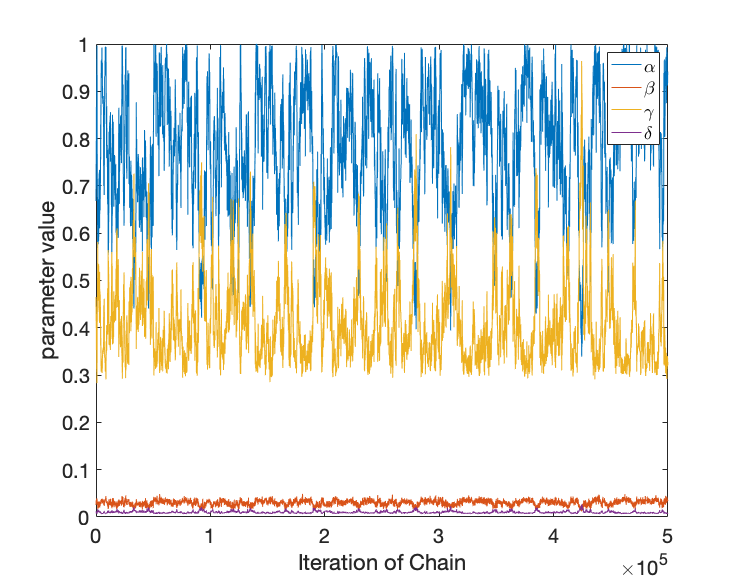
\includegraphics[width=15cm]{MCMC_figs/met_lv_final/final_mh_chain.png}
    \caption{Trace plot for the sampling chain (500,000 samples) for the DRAM MCMC parameterization of the Lotka-Volterra model. Each line shows the sampled parameter values. This figure visualizes each parameter value that has been sampled and accepted that will be used to build parameter PDFs. This chain visualization shows us that the algorithm is having a some difficult determining the most suitable mean as we see a distinct ``wave" pattern which indicates that chain mixing could be improved.}
    \label{fig:2mcmc}
\end{figure}
 In Figure \ref{fig:2mcmc}, we illustrate the final 500,000 values that our algorithm sampled. From a visual perspective, we can see that the chains appear to have achieved a steady-state; although the values still ``jump" up and down, they appear to do so around a certain value. For instance, $\alpha$ appears to move around 0.8 while $\gamma$ settles around 0.4. Often such a visual analysis of the chain as in Figure \ref{eq:2mcmc} is used to evaluate a chain's \textit{mixing time}. Briefly, mixing time refers to number of samples a chain requires to achieve a steady state and is directly related to the performance of the algorithm \cite{mixingtime}. Thus, a well-mixed chain is such a chain that in the given number of samples has achieved a steady state while a poorly mixed chain has not. Figure \ref{fig:2mcmc} demonstrates that the chain is fairly well mixed however as we will see later, it could be improved.
 \par The chain's ability to reach a steady state is important in determining the reliability of the final parameter distributions. We want our chain to reach a steady state or \emph{converge} by the time we complete sampling as this indicates the algorithm could not find ``better" or more likely values for the parameters within the constraints of the model. A \textit{burn-in} period gives the algorithm time to explore the parameter space and converge before sampling and collection for the distribution begins.
\par There are several formal techniques for confirming chain convergence, for example the Geweke diagnostic \cite{geweke1} and the Gelman-Rubin diagnostic \cite{gelman_rubin}. We use the Geweke diagnostic to quantitatively assess convergence. Next, let's look at the statistical results from our chain in Table \ref{tab:1mcmc}.
\begin{table}[H]
\centering
        \begin{tabular}{c c|c c |c c ||c}
            \hline
            \textbf{Parameter} & \textbf{Initial Value} & \textbf{Mean} & \textbf{Std} &  \textbf{Geweke} & \textbf{p-value} & \textbf{Chain Acceptance Rate}\\ 
            \cline{1-7}
            $\alpha$ & 0.625 & 0.779 & 0.134 & -0.1325 & 0.895 & \multirow{4}{*}{0.0242} \\
            $\beta$ & 0.190 & 0.0301 & 5.40e-03 & -0.1177 & 0.906\\
            $\gamma$ & 0.661 & 0.412 & 0.0871 & 0.1199 & 0.905\\
            $\delta$ & 0.0468 & 9.95e-03 & 2.30e-03 & 0.1226 & 0.902 
            \\\hline
                          \hline
        \end{tabular}
    \caption{Table listing results of the Metropolis chain. Parameter means, standard deviations, convergence diagnostics (Geweke), and the Geweke p-values are calculated. Based on the p-values values, the chain has converged for all the parameters. The chain acceptance rate is significantly less than 25\% indicating that the algorithm was likely rejecting many candidates. This makes it more likely for the algorithm to have gotten stuck in a local maximum.}
    \label{tab:1mcmc}
\end{table}
From Table \ref{tab:1mcmc}, we are most interested in the Geweke diagnostic. For now, it is enough to know that the diagnostic compares the means of the first $10\%$ and last $50\%$ of the chain. If these means are similar, it indicates that convergence occurred within the first $10\%$ of the chain's samples \cite{geweke_ppt} \cite{geweke1}. In this implementation, the Geweke value is calculated as a two-sample Z-test and a p-value is derived from the z-value. Some basic statistical knowledge is necessary to calculate and interpret the Geweke diagnostic which we explore in Appendix \ref{appendix:gewekediagnostic}. To determine convergence, we analyze the p-values. Briefly, p-values indicate evidence against a null hypothesis. In this scenario our null hypothesis is that our chain has converged (and our alternative is that the chain has not converged). The smaller the p-value, the more evidence we have to reject the null hypothesis, that is to say that it is unlikely that the chain has converged. We will use the typical p-value of 0.05 to indicate rejection of the null hypothesis. By this standard we \textit{fail} to reject our null hypothesis, thus we say that the chain has converged for all our parameters and we are confident that the parameters' mean values produce a good prediction of our model (as seen in Figure \ref{fig:5mcmc}). 
\par Finally, we can assess the performance using the chain acceptance ratio. Previous literature mathematically justifies that an acceptance rate of around $25\%$ indicates high performance of the chain \cite{convergence} \cite{converge_threshold}. However, it should be cautioned that (as with most claims of universal applications), we cannot rely solely on this diagnostic. We merely present the chain acceptance rate as one mode of investigating chain performance. An acceptance rate of 0.0242, is significantly smaller than the recommended 0.25. This indicates that our algorithm is perhaps not performing very well. With such a low acceptance rate, our algorithm seems to have rejected a majority of the candidate parameter sets. This increases the probability that the algorithm has either found a local maximum or gotten stuck in one. Due to the convergence we see using the Geweke p-values, we hypothesize that our algorithm is doing the former. A visual assessment of the mixing of the chain in Figure \ref{fig:2mcmc} seems to corroborate this idea. A well-mixed chain is defined as having explored all important regions within its stationary distribution \cite{convergence_mixing}. Visually at each sample, we want to see our chain explore the full range (given by the implementer) of the parameter value, settling around a mean value \cite{convergence_ppt}. In looking at the trace plot for $\alpha$, we see that while the chain changes values at each step, the amount by which parameter values change differs sample to sample. This results in a pronounced increase and decrease of mean (although it does still converge around a single value). In a well-mixed chain (see Figure \ref{fig:7mcmc}), we would see that parameter values differ by a very similar amount sample to sample.
Other methods for formally assessing mixing are beyond the scope of this paper \cite{convergence_mixing}.
\par The \texttt{mcmcstat} library provides functions to analyze the relationships between the parameters of our model.
\begin{figure}[H]
    \centering
    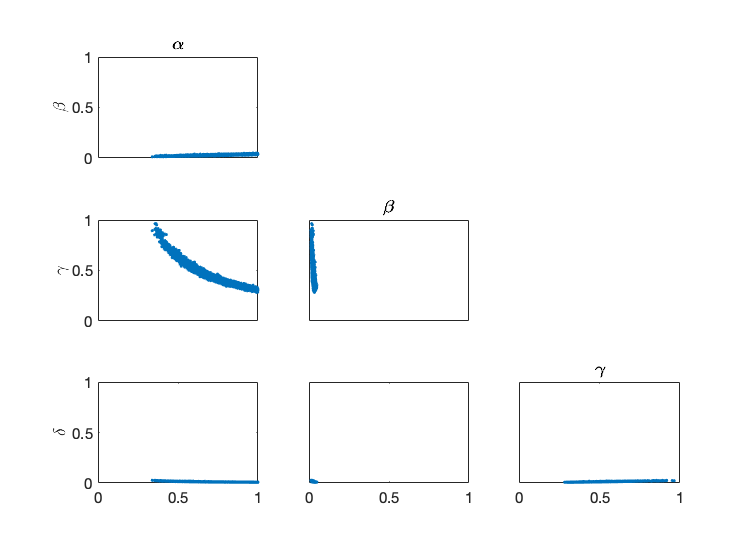
\includegraphics[width=15cm]{MCMC_figs/met_lv_final/final_mh_samples.png}
    \caption{Relationships between Lotka-Volterra parameter values per chain sample using the Metropolis MCMC algorithm. All x- and y-axes are of the same same scale respectively. Most notably there is a clear negative relationship between $\alpha$ and $\gamma$. This correlation will play a role in the algorithm's ability to choose optimal parameter values.}
    \label{fig:3mcmc}
\end{figure}
Recall that the parameter space for this model is 4-dimensional. Figure \ref{fig:3mcmc} illustrates the relationships in our parameter space as more and more values are sampled. We can see that the $\alpha \sim \gamma$ relationship is clearly negative. Recall the mirror relationship that we saw in the trace plots of these parameters in Figure \ref{fig:1mcmc}. Figure \ref{fig:3mcmc} confirms this relationship that we saw and that $\alpha$ and $\gamma$ are correlated. Ideally, we would like to see a normal clustering of values with no clear correlation. While the correlation between parameter values are a result of the model, they do impact the sampling procedure as strong correlations make it difficult to determine unique parameter sets. While we will not explore this idea of \emph{parameter identifiability} in this tutorial, we encourage the reader to consult \cite{smithCh8}. Briefly, parameter identifiability quantifies how parameter values may be correlated but can still be uniquely determined by the model \cite{smithCh8}.
\paragraph{Working with the distributions}
\par Now let's see how we can determine a posterior distribution for our parameters:
\begin{figure}[H]
    \centering
    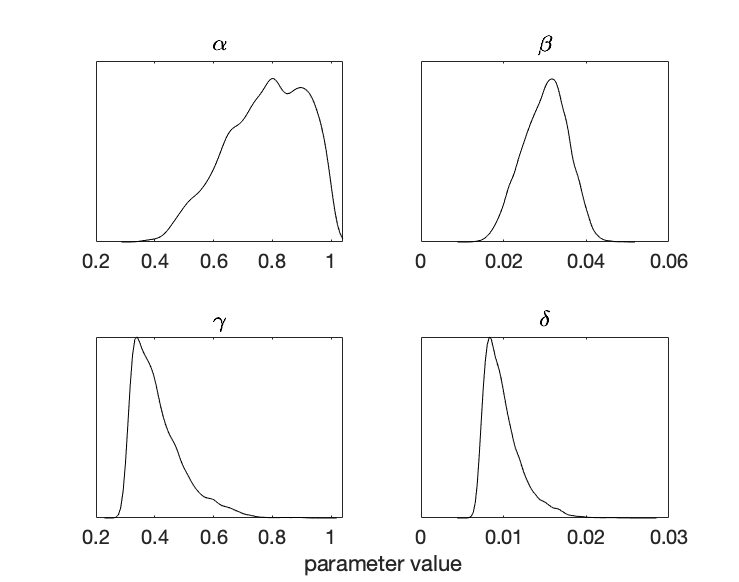
\includegraphics[width=15cm]{MCMC_figs/met_lv_final/final_mh_den.png}
    \caption{Posterior density distributions for each Lotka-Volterra model parameter using the Metropolis MCMC algorithm. The distribution for $\alpha$ is noticeably not smooth at its peak. This illustrates the algorithm's inability to find the optimal mean value for $\alpha$. Additionally, this non-smoothness is reflected in the lower Geweke value, which although indicates convergence, does not indicate such complete convergence as the other parameters.}
    \label{fig:4mcmc}
\end{figure}
By collecting the accepted values for each parameter, we can fit distributions such as those in Figure \ref{fig:4mcmc}. While we cannot definitively categorize these distributions visually, we can see that at least $\gamma$ and $\delta$ resemble some a familiar distribution, namely a lognormal distribution. It is more difficult to categorize $\alpha$ although $\beta$ appears to tend toward a normal distribution. It is useful to visualize these distributions, but they may not be directly useful. However, we can calculate their means that may be used in computations. Additionally, we make note of the relative ``bumpiness" of the peak in $\alpha$'s PDF. This indicates that the algorithm may have had difficulty in pinpointing the optimal mean value. To understand why the algorithm may have struggled to estimate $\alpha$, recall the hare population in Figure \ref{fig:0prob}. In the earlier data, the hare population has rather large spikes in population growth and the peaks around 1850 and 1870 have what appears to be 2 peaks. As the likelihood function is implemented as a sum of squares function that depends directly on the raw data, the irregularity of the data may have made it difficult for the Metropolis algorithm to pinpoint the hare population increase rate.  The lack of smoothness is also reflected in $\alpha$'s lower Geweke value; although we still conclude convergence of the chain for $\alpha$, the chain did not demonstrate the confidence of convergence as it did for the remaining 3 parameters. Next we visualize some predictions of our model using the chain samples.
\begin{figure}[H]
    \centering
    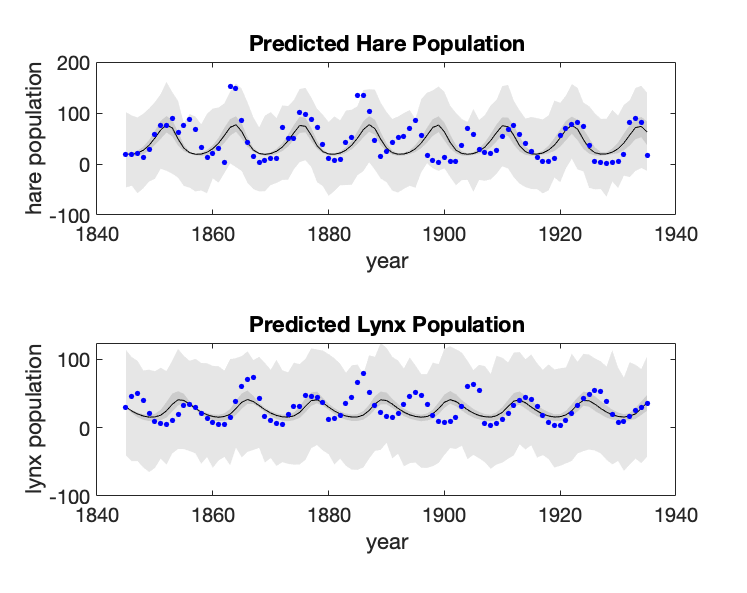
\includegraphics[width=15cm]{MCMC_figs/final_mh_modpred.png}
    \caption{Predicted hare and lynx populations using parameter values found using Metropolis MCMC. Black lines indicate the mean model prediction; gray area indicates 95$\%$ probability limits for new observations; blue points indicate original raw hare and lynx population data. For both hare and lynx populations, the Metropolis parameterization is unable to fully capture the irregular peaks in populations that occur from around 1840 to 1910. Instead, we see a symmetric periodic function for both population predictions.}
    \label{fig:5mcmc}
\end{figure}
From Figure \ref{fig:5mcmc}, we can get a visual sense of how well our sampled parameter values predict the raw data given our model. In the predicted lynx population, all of the raw data falls within our $95\%$ probability range, which tells us our predictions are doing a good job of capturing the data. In the hare population, most of the raw data falls within that $95\%$ range, although few points do not. The 95\% probability ranges help us to determine how well a majority of our sampled parameter sets capture the data. However in practice, we are most interested in the prediction that uses the mean parameter values as we are likely to only want to use a single set of parameter values in future models.
\subsection{Delayed Rejection Adaptive Metropolis} \label{Delayed_Rejection_Adaptive_Metropolis}
There are many variations of MCMC methods that can be used to parameterize biological systems, each with their own benefits. We have chosen to describe the delayed rejection adaptive Metropolis (DRAM) MCMC method to compare with the Metropolis MCMC algorithm \cite{DRAM1}. As its name suggests, DRAM builds upon several of the MCMC algorithms namely adaptive Metropolis (AM) and delayed rejection (DR) and is often used in order to allow for better adaptation of the sampling chain as time goes on \cite{DRAM1}. Like most MCMC methods, DRAM requires initialization of proposal, likelihood, and prior distributions. However, while the proposal distribution of Metropolis MCMC is assumed (via a covariance matrix) given some \emph{a priori} information about parameter values and variability, in adaptive methods such as DRAM, posterior information learned during the progression of the algorithm is immediately incorporated and the algorithm adjusted. In order to understand the DRAM algorithm, it is useful to begin with its two parts.
\subsubsection{Adaptive Metropolis}
The adaptive Metropolis method is an optimization of of simpler MCMC algorithms as it allows the algorithm to move quickly through parameter space of low probability \cite{collis}, \cite{adaptive_andrieu}. The adaptive algorithm does this by updating its proposal distribution as sampling occurs thus creating a more informed pool from which candidates are drawn. The adaptive Metropolis algorithm proceeds as follows:
\begin{tcolorbox} \label{box:am}
\textbf{\underline{Adaptive Metropolis Algorithm (with an uninformative prior)}}
\begin{enumerate}
\item Set number samples to take, $N$; number of candidates to sample before updating the proposal distribution, $k_0$; and burn-in period, $k_b$
    \item Determine an initial parameter guess $\theta^0 = argmin_q \sum_{i=1}^{n}[M_i - f_i(\theta)]^2]$
    \item Set $SS_{\theta^0} = \sum_{i = 1}^{n}[y_i - f_i(\theta^0)]^2$ (for likelihood)
    \item Compute an initial variance estimate $s_0^2 = \frac{SS_{\theta^0}}{n-p}$ ($n =$ number of data points, $p = $ number of parameters)
    \item Construct an initial proposal covariance matrix $V_0$ 
    \item For each iteration of the chain, $k = 1,...,N$
    \begin{enumerate}
        \item Sample $z \sim N(0,I_p)$
        \item Construct candidate $\theta^* = \theta^{k-1}+ V_0z$
        \item Compute $SS_{\theta^*} = \sum_{i = 1}^{n}[y_i - f_i(\theta^*)]^2$ (likelihood sum of squares)
        \item Compute acceptance criterion
            \begin{center}
                $\alpha(\theta^* | \theta^{k-1}) = min(1, e^{-[SS_{\theta^*}-SS_{\theta^{k-1}}/2s_{k-1}^2]})$
            \end{center}
        \item Accept $\theta^*$ with a probability 1 if $\alpha \geq 1$ and accept it with probability $\alpha$ if $\alpha < 1$.
        \begin{itemize}
            \item If $\theta^*$ is accepted
            \begin{center}
                $\theta^k = \theta^*$, $SS_{\theta^k} = SS_{\theta^*}$
            \end{center}
            \item Else
            \begin{center}
                $\theta^k = \theta^{k-1}$, $SS_{\theta^k} = SS_{\theta^{k-1}}$
            \end{center}
        \end{itemize}
        \item If $k > k_b$ collect $\theta^*$ in posterior matrix $P$, else discard
        \item Update $s_k^2 = \frac{SS_{\theta^k}}{n-p}$
    \end{enumerate}
    \begin{tcolorbox}[colback=red!5,colframe=red!75!black,title=Adaptive Step]
    \item If $k = k_0$ adaptation commences: the initial $V_0$ is updated to the covariance matrix, $V_{k}$ \label{step:7adapt}
    \begin{center}
       $V_{k} = s_{p}cov(\theta^{0},\theta^{1},...,\theta^{k-1}) + \epsilon I_{p}$
    \end{center}
    \end{tcolorbox}
    
\end{enumerate}
\emph{Based on Smith (2014) Algorithm 8.8}
\end{tcolorbox}
\par We want to choose $k_0$ to balance a mixing with sufficient diversity of points to ensure a non-singular covariance matrix ($V$). Note that $V$ must be non-singular (i.e. invertible) because the calculating the proposal distribution requires computing $V$'s inverse \cite{WallinBolin2018nonsingcov}. Shorter adaptation intervals tend to produce better mixing and higher acceptance ratios \cite{convergence_mixing} and thus, the chain is more responsive to new data from parameter space not previously explored. In practice, $k_0$ is often 100 \cite{smithCh8}. 
\par The fundamental steps of the AM algorithm are taken directly from the Metropolis algorithm, in both algorithms sample, accept, and reject candidate parameter sets in the same way. Recall from the Metropolis algorithm that in Step 6a $z$ is the random component of selecting a parameter set and is what makes each $\theta^*$ unique even if multiple $\theta^*$s are found using the same $\theta^{k-1}$. Step \ref{step:7adapt} of this algorithm is the adaptive step of the AM algorithm. This step updates the current covariance matrix $V_0$ according to the covariances between the accepted parameter sets. Here, $s_{p}$ is a design parameter that depends on the dimension ($p$) of the parameter space; a common choice is $s_{p} = 2.38^{2}/p$ \cite{smithCh8}. The term $\epsilon I_{p}$ refers to an identity matrix of dimension $p$-by-$p$ (to ensure $V_{k}$ is positive definite). Often, $\epsilon = 0$ \cite{smithCh8}.
\par While Steps 1-6 are directly adapted from the Metropolis MCMC algorithm, Step 7 in the above algorithm is the new adaptive step that allows the algorithm to traverse parameter space of lower probability efficiently.

\subsubsection{Delayed Rejection}
\par The delayed rejection MCMC improves the efficiency of other MCMC methods by increasing the transition probability of parameters leading to improvement in chain mixing \cite{trias2009delayed}. In the standard Metropolis algorithm, when a candidate parameter set $\theta^*$ is rejected (with its prescribed acceptance ratio $\alpha$), the current step parameter set, $\theta^{k-1}$, is retained and $\theta^*$ is discarded before choosing the next sample. In the \emph{delayed rejection} (DR) algorithm, when $\theta^*$ is rejected, alternative candidates $\theta^{*j}$ are constructed and considered instead of immediately reverting back to $\theta^{k-1}$. We can specify the number of alternatives our algorithm will propose before moving on to the next iteration of the chain. By sampling multiple candidates under the same sampling conditions (recall Step \ref{step:6met}g of the Metropolis algorithm) we allow the algorithm to consider parameter space with lower probability that, in the Metropolis algorithm, may have been omitted. Additionally, these alternative candidates prevent the algorithm from getting stuck in local maxima or minima. Loosely this works as follows: when we accept a candidate parameter, its values become the basis of constructing the next proposed candidate (recall \textbf{Steps \ref{step:6met}a} and \textbf{\ref{step:6met}b} of the Metropolis algorithm). Therefore, the next time we reject a candidate, the subsequent candidate must be constructed using only the same information as the most recently accepted parameter set. This is computationally inefficient as we have already searched this particular parameter space, yet we are forced to draw again from the same space and in effect, we have not explored anything new. When this immediate rejection process is compounded, we may encounter long periods in which we propose many candidates only using a single set of parameter values, thus we are not exploring the whole parameter space and run the risk of staying in local maxima.
\par In order to work with alternative candidates, we must redefine the acceptance criterion, $\alpha$. We follow an explanation from \cite{smithCh8}.\\
For example, $\theta^{*2}$, a second-stage candidate, is chosen using proposal function
\begin{equation} \label{eq:17mcmc}
J_{*2}(\theta^{*2}|\theta^{k-1},\theta^*) \sim N(\theta^{k-1}, \gamma^2V)
\end{equation} 
where $V$ is the covariance matrix informing the proposal distribution. $J_{*2}(\theta^{*2}|\theta^{k-1},\theta^*)$ indicates that we propose $\theta^{*2}$ having started at $\theta^{k-1}$ and rejected $\theta^*$. Finally, $\gamma < 1$ tunes the second-stage proposal function and increases mixing \cite{smithCh8}. The acceptance criteria for the second-stage candidate thus is\\
\begin{equation} \label{eq:18mcmc}
\alpha_{*2}(\theta^{*2}|\theta^{k-1}, \theta^*) = min(1, \frac{P(\theta^{*2}|M)J(\theta^*|
    \theta^{*2})[1-\alpha(\theta^*|\theta^{*2})]}{P(\theta^{k-1}|M)J(\theta^*|\theta^{k-1})[1-\alpha(\theta^*|\theta^{k-1})]})
\end{equation}
With these additional steps, we outline the DR algorithm.
\begin{tcolorbox} \label{alg:DRmcmc}
\textbf{\underline{Delayed Rejection Algorithm (with an uninformative prior)}}
\begin{enumerate}

\item Set number samples to take, $N$; choose number of alternatives, $n_{alt}$; and determine a burn-in period, $k_b$
    \item Determine an initial parameter guess $\theta^0 = argmin_q \sum_{i=1}^{n}[M_i - f_i(\theta)]^2]$
    \item Set $SS_{\theta^0} = \sum_{i = 1}^{n}[y_i - f_i(\theta^0)]^2$ (for likelihood)
    \item Compute an initial variance estimate $s_0^2 = \frac{SS_{\theta^0}}{n-p}$ ($n =$ number of data points, $p = $ number of parameters)
    \item Construct a proposal covariance matrix $V$ 
    \item For each iteration of the chain, $k = 1,...,N$
    \begin{enumerate}
        \item Sample $z \sim N(0,I_p)$ 
        \item Construct candidate $\theta^* = \theta^{k-1}+ V_0z$
        
        \item Compute $SS_{\theta^*} = \sum_{i = 1}^{n}[y_i - f_i(\theta^*)]^2$ (likelihood sum of squares)
        \item Compute acceptance criterion
            \begin{center}
                $\alpha(\theta^* | \theta^{k-1}) = min(1, e^{-[SS_{\theta^*}-SS_{\theta^{k-1}}/2s_{k-1}^2]})$
            \end{center}
        \item Accept $\theta^*$ with a probability 1 if $\alpha \geq 1$ and accept it with probability $\alpha$ if $\alpha < 1$.
        \begin{enumerate}
            \item If $\theta^*$ is accepted, proceed to next sample
            \begin{center}
                $\theta^k = \theta^*$, $SS_{\theta^k} = SS_{\theta^*}$
            \end{center}
            \begin{tcolorbox}[colback=red!5,colframe=red!75!black,title=Delayed Rejection]
        
            \item Else enter \textbf{delayed rejection process} while $n_i \leq n_{alt}$
            \begin{enumerate}
                \item Set design parameter $\gamma < 1$
                \item Sample $z_{n_i} \sim N(0,I_p)$ 
                \item Construct i-stage alternative $\theta^{*i} = \theta^{k-1} + \gamma Vz_{n_i}$
                \item Compute acceptance criterion
                \begin{center}
                  $\alpha_{*i}(\theta^{*i}|\theta^{k-1}, \theta^*) = min(1, \frac{P(\theta^{*i}|M)J(\theta^*|
    \theta^{*i})[1-\alpha(\theta^*|\theta^{*2})]}{P(\theta^{k-1}|M)J(\theta^*|\theta^{k-1})[1-\alpha(\theta^*|\theta^{k-1})]})$
                \end{center}
                \item Accept $\theta^{*i}$ with a probability 1 if $\alpha_{*i} \geq 1$ and accept with probability $\alpha_{*i}$ if $\alpha_{*i} < 1$.
            \end{enumerate}
            \end{tcolorbox}
        \end{enumerate}
        \item If $k > k_b$ collect $\theta^*$ in posterior matrix $P$, else discard
        \item Update $s_k^2 = \frac{SS_{\theta^k}}{n-p}$
    \end{enumerate}
\end{enumerate}
\emph{Based on Smith (2014) Algorithm 8.8}
\end{tcolorbox}
In Step 1, we can choose to determine a specific number of alternative parameter sets that the algorithm will propose, $n_alt$, before rejecting and proceeding to the next iteration of the algorithm. Note that if the algorithm is allowed to propose infinite alternatives, the efficiency of the algorithm is likely to increase (possible to infeasible levels). In Step 6e.ii we see the delayed rejection process. This process is very similar to the Metropolis method of accepting and rejecting candidate parameter sets. In Step 6e.ii.B we see that again we have $z_{n_i} \sim N(0, I_p$ which is the random component of selecting a parameter set and is what makes each $\theta^*i$ unique as each alternative candidate is sampled using the same $\theta^{k-1}$.
\par Now we have an understanding of both the delayed rejection and adaptive Metropolis MCMC algorithms, we can construct the final DRAM algorithm. We will do this in the following section by using Steps 1-6 of the Metropolis algorithm as a foundation and incorporating Step 7 of the adaptive Metropolis algorithm and Step 6e(ii) of the delayed rejection algorithm.
\subsubsection{Constructing the DRAM Algorithm}
Now that we have the basis for the two components of the delayed rejection adaptive Metropolis algorithm, all that is left to do is merge them. Using the foundation of the Metropolis algorithm, we add an adaptive step and a delayed rejection process. In the DRAM algorithm, the adaptive Metropolis and delayed rejection work together: AM updates the proposal via previously accepted candidates and the covariance matrix and DR alters the proposal function to improve mixing.
\begin{tcolorbox}
\textbf{\underline{The DRAM Algorithm (with an uninformative prior)}} 
\begin{enumerate}
\item Set number of samples to take, $N$, adaptive chain length, $k_0$, number of alternatives, $n_{alt}$, and burn-in period, $k_b$
    \item Determine an initial parameter guess $\theta^0 = argmin_q \sum_{i=1}^{n}[M_i - f_i(\theta)]^2]$
    \item Set $SS_{\theta^0} = \sum_{i = 1}^{n}[y_i - f_i(\theta^0)]^2$ (for likelihood)
    \item Compute an initial variance estimate $s_0^2 = \frac{SS_{\theta^0}}{n-p}$ ($n =$ number of data points, $p = $ number of parameters)
    \item Construct an initial covariance matrix $V_0$ 
    \item For each iteration of the chain, $k = 1,...,N$
    \begin{enumerate}
        \item Sample $z \sim N(0,I_p)$
        \item Construct candidate $\theta^* = \theta^{k-1}+ V_0z$
        \item Compute $SS_{\theta^*} = \sum_{i = 1}^{n}[y_i - f_i(\theta^*)]^2$ (likelihood sum of squares)
        \item Compute acceptance criterion
            \begin{center}
                $\alpha(\theta^* | \theta^{k-1}) = min(1, e^{-[SS_{\theta^*}-SS_{\theta^{k-1}}/2s_{k-1}^2]})$
            \end{center}
        \item Accept $\theta^*$ with a probability 1 if $\alpha \geq 1$ and accept it with probability $\alpha$ if $\alpha < 1$.
        \begin{tcolorbox}[colback=red!5,colframe=red!75!black,title=DRAM Step]
        \begin{enumerate}
            \item If $\theta^*$ is accepted, proceed to next sample
            \begin{center}
                $\theta^k = \theta^*$, $SS_{\theta^k} = SS_{\theta^*}$
            \end{center}
            \item Else enter \textbf{delayed rejection process} while $n_i \leq n_{alt}$
            \begin{enumerate}
                \item Set design parameter $\gamma < 1$
                \item Sample $z_{n_i} \sim N(0,I_p)$ 
                \item Construct i-stage alternative $\theta^{*i} = \theta^{k-1} + \gamma Vz_{n_i}$
                \item Compute acceptance criterion
                \begin{center}
                  $\alpha_{*i}(\theta^{*i}|\theta^{k-1}, \theta^*) = min(1, \frac{P(\theta^{*i}|M)J(\theta^*|
    \theta^{*i})[1-\alpha(\theta^*|\theta^{*2})]}{P(\theta^{k-1}|M)J(\theta^*|\theta^{k-1})[1-\alpha(\theta^*|\theta^{k-1})]})$
                \end{center}
                \item Accept $\theta^{*i}$ with a probability 1 if $\alpha_{*i} \geq 1$ and accept with probability $\alpha_{*i}$ if $\alpha_{*i} < 1$.
            \end{enumerate}
            
        \end{enumerate}
        \item If $k = k_0$ adaptation commences: the initial $V_0$ is updated to the covariance matrix, $V_{k}$
       
        \begin{center}
            $V_{k} = s_{p}cov(\theta^{0},\theta^{1},...,\theta^{k-1}) + \epsilon I_{p}$
        \end{center}
        \end{tcolorbox}
        \item If $k > k_b$ collect $\theta^*$ in posterior matrix $P$, else discard
        \item Update $s_k^2 = \frac{SS_{\theta^k}}{n-p}$
        
    \end{enumerate}
    
\end{enumerate}
\emph{Based on Smith (2014) Algorithms 8.8 and 8.10}
\end{tcolorbox}
We have now combined the adaptive Metropolis and delayed rejection processes outlined in Steps 6e and 6f. In the next section we will estimate parameters for the Lotka-Volterra system and compare results with the Metropolis MCMC parameterization.

\subsubsection{Parameterizing Lotka-Volterra}
As with the Metropolis MCMC, DRAM was used to estimate parameters of the Lotka-Volterra system. We implemented likelihood, and proposal distributions identical to those used in the Metropolis parameterization (Steps 3 and 5). We implemented a log-uniform prior function, however we used a different range for each parameter value (see Table \ref{table:ParameterNotationAppendix} in Appendix \ref{general_appendix}). The number of iterations was also held constant, the adaptive interval $k_0$ was defined to be 100, a common default in DRAM, and 2 alternate candidates were specified (this number is a default setting of the MATLAB \texttt{mcmcstat} library function \texttt{mcmcrun}; Step 1). Just as in the Metropolis parameterization, we first visualize the burn-in and sampled chains.
\begin{figure}[H]
    \centering
    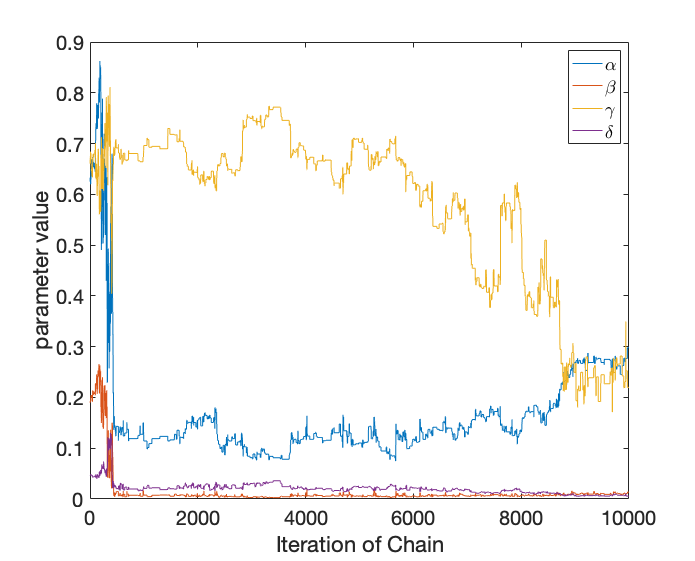
\includegraphics[width=15cm]{MCMC_figs/met_lv_final/final_dram_burninchain.png}
    \caption{Burn-in chain (10,000 samples) for the DRAM MCMC parameterization of the Lotka-Volterra model. Each line shows the sampled parameter values. This figure illustrates the movement of the Markov chain as it samples parameters with the goal of finding the most likely range of values. As expected, the chain has not converged for all the parameters yet.}
    \label{fig:6mcmc} 
\end{figure}
\begin{figure}[H]
    \centering
    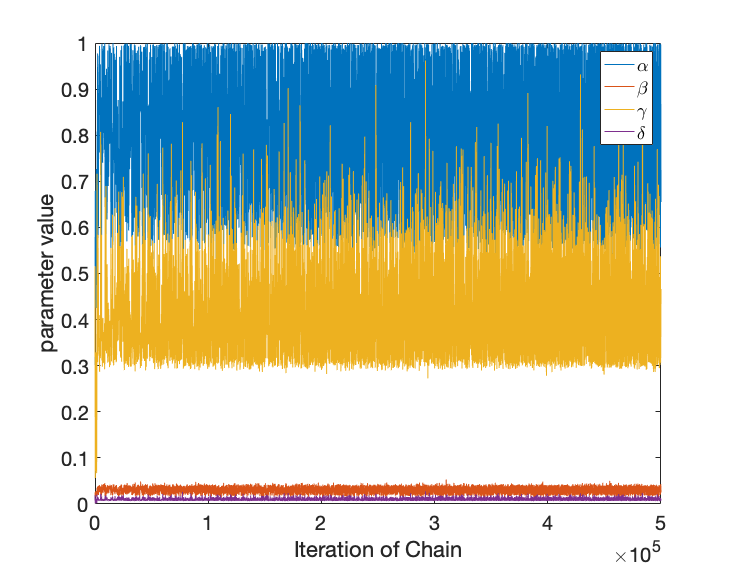
\includegraphics[width=15cm]{MCMC_figs/met_lv_final/final_dram_chain.png}
    \caption{Sampling chain (500,000 samples) for the DRAM MCMC parameterization of the Lotka-Volterra model. Each line shows the sampled parameter values. This figure visualizes each parameter value that has been sampled and accepted that will be used to build parameter PDFs. This chain visualization shows a ``fuzzy caterpillar" sampling pattern indicative of a well-mixed chain.}
    \label{fig:7mcmc}
\end{figure}
Figure \ref{eq:6mcmc} shows the chain's exploration of the parameter space during the burn-in period (10,000 samples). From a preliminary visual analysis of this chain, we can see that $\alpha$, $\beta$, and $\delta$ seem to find their steady states fairly quickly ($<$ 2,000 samples). Additionally, $\gamma$ seems to trend toward its optimal value range more immediately than in the Metropolis algorithm (Figure \ref{fig:1mcmc}). From 0 to around 9,000 samples, $\gamma$ generally trends downward until it hits a value range of $0.3$ to $0.2$. In Figure \ref{fig:7mcmc}, we illustrate the final 500,000 values that our algorithm sampled. From a visual perspective, this chain appears to demonstrate good mixing as the chain appears to have settled in a steady state for each parameter. This is evidenced by the lack of a ``wave" pattern that we saw in Figure \ref{fig:2mcmc} and thus, a lack of increasing or decreasing trends of parameter values. For instance, $\alpha$ appears to move around 0.8 while $\gamma$ settles around 0.4. Statisticians have often referred to a well-mixed plot as resembling a ``fuzzy caterpillar", due to its dense and somewhat spiked appearance \cite{fuzzy_caterpillar}. However, the means of these well-mixed plots are relatively constant mean and suggest that the values of the chain are no longer changing and are therefore in a steady state.
\par Next, let's look at the statistical results from our chain in Table \ref{tab:2mcmc}.
%           
\begin{table}[H]
\centering
        \begin{tabular}{c c |c c | c c ||c}
            \hline
            \textbf{Parameter} & \textbf{Inital Value} & \textbf{Mean} &  \textbf{Std} & \textbf{Geweke} & \textbf{p-value} & \textbf{Chain Acceptance Rate}\\ 
            \cline{1-7}
            $\alpha$ & 0.625 & 0.787 & 0.139 & 0.0219 & 0.983 & \multirow{4}{*}{0.241} \\
            $\beta$ & 0.190 & 0.0303 & 5.58e-03 & 0.0136 & 0.989\\
            $\gamma$ & 0.661 & 0.407 & 0.0908 & -0.0867 & 0.931\\
            $\delta$ & 0.0468 & 9.83e-03 & 2.39e-03 & -0.0838 & 0.933
             \\\hline
                          \hline
                           
        \end{tabular}
    \caption{Table listing results of the DRAM chain. Parameter means, standard deviations, the convergence diagnostic (Geweke), and the Geweke p-values are calculated. Based on the Geweke p-values values, we conclude that the chain has converged for all the parameters. The chain acceptance rate is very close to the 25\% threshold indicating that the algorithm was able to effectively search the parameter space.}
    \label{tab:2mcmc}
\end{table}
We can use the parameter means and standard deviations to find the optimal range of parameter values for this model. We look to the Geweke p-values to quantitatively determine convergence. We see that all of our p-values are greater than 0.05 and thus we fail to reject the null hypothesis that the chain has converged.
Thus we say that the chain has converged for all our parameters and we are confident that the parameters' mean values produce a good prediction of our model (as seen in Figure \ref{fig:10mcmc}). Lastly, we look at the chain's acceptance ratio 
\par We look again to the chain's acceptance rate and the visual assessment of mixing to help us analyze the chain's performance. In Table \ref{tab:2mcmc}, we see that the acceptance rate is very close to the proposed indication of good performance, $25\%$ acceptance. This leads us to believe that our chain was able to effectively search the parameter space. Intuitively, we expect the DRAM method to have a higher acceptance rate than the Metropolis method because we are able to propose several alternative candidates instead of immediately rejecting a sample. This increases the probability of accepting at any iteration of the algorithm. We further validate this belief by looking at the trace plots of the chains in Figure \ref{fig:7mcmc}. Figure \ref{fig:7mcmc} shows us that our chain is well-mixed for each of our parameters as it appears our chain has reached a steady-state for each parameter value. 
\par Let's look at the relationships between parameters as the chain samples.
\begin{figure}[H]
    \centering
    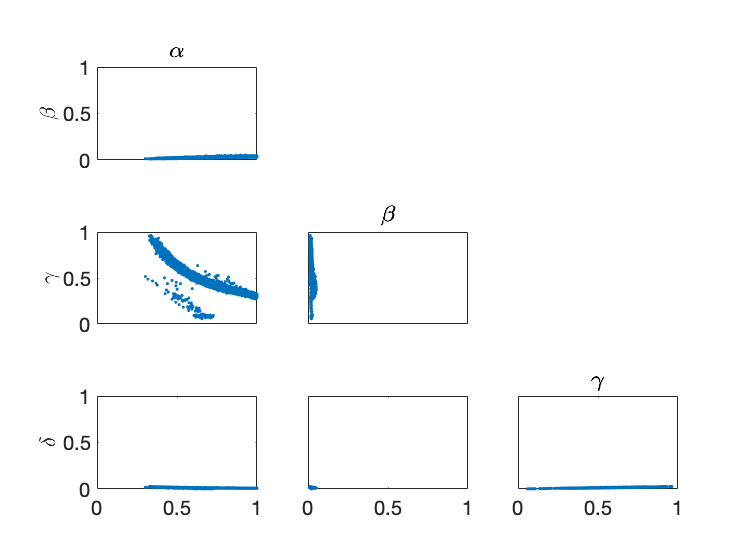
\includegraphics[width=15cm]{MCMC_figs/met_lv_final/final_dram_samples.png}
    \caption{Correlations between Lotka-Volterra parameter values per chain sample using the DRAM MCMC algorithm. There is a clear negative correlation between $\alpha$ and $\gamma$. Recalling the idea of \textit{parameter identifiability}, this may have an impact on algorithm's sampling ability.}
    \label{fig:8mcmc}
\end{figure}
Similarly to the correlation that we saw in Figure \ref{fig:3mcmc}, $\alpha$ and $\gamma$ have a strong negative relationship. However, we see what appears to be two clusters within the $\alpha \sim \gamma$ plot. This indicates that perhaps the algorithm had discovered two local maxima. However, we saw that the $\alpha$'s Geweke diagnostic from the DRAM parameter estimation was greater than the Metropolis diagnostic, indicating a higher confidence in convergence. Due to the sampling methodology of the DRAM algorithm, we hypothesize that the cluster with more samples is the global maximum and the other cluster may be a local maximum.
\paragraph{Working with the distributions}
We visualize the posterior PDFs for the system's parameters:
\begin{figure}[H]
    \centering
    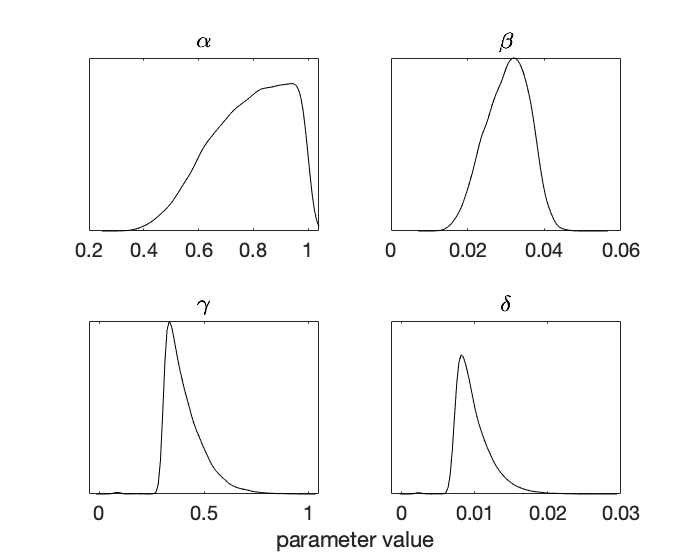
\includegraphics[width=15cm]{MCMC_figs/met_lv_final/final_dram_den.png}
    \caption{Posterior density distribution for each Lotka-Volterra parameter using the DRAM MCMC algorithm. Unlike the PDFs produced by the Metropolis MCMC algorithm, these PDFs appear fairly smooth. This indicates that the algorithm was more successful at finding global maxima.}
    \label{fig:9mcmc}
\end{figure}
We will perform a more thorough comparison of the two MCMC algorithms, but for now, we can see that like the Metropolis MCMC algorithm, we produce posterior density functions for each parameter in our model. We note that the $\alpha$ distribution appears smoother than its distribution produced by the Metropolis algorithm, this corroborates our earlier analyses of clear convergence and the location of a global maximum. Similarly to the Metropolis PDFs, we cannot strictly classify these distributions as normal. Instead, we can see how these sampled parameter sets perform against our original data.
\begin{figure}[H]
    \centering
    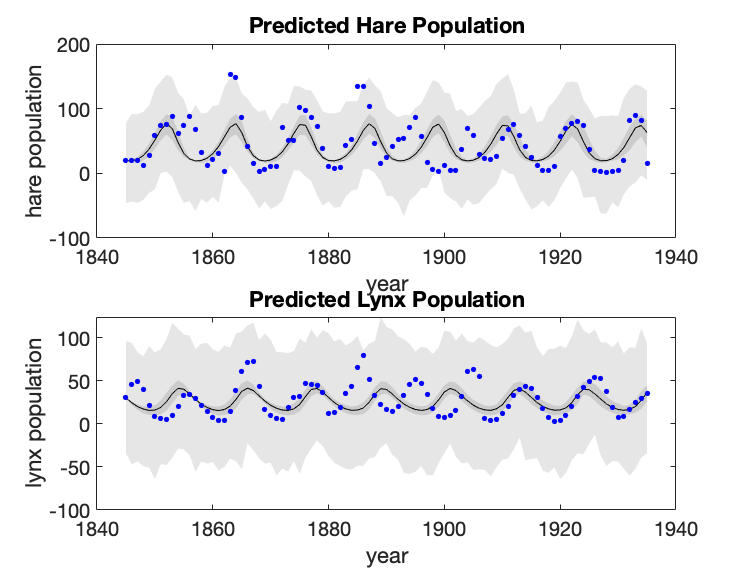
\includegraphics[width=15cm]{MCMC_figs/final_dram_modpred.png}
    \caption{Predicted hare and lynx populations using parameter values found using DRAM MCMC. Black lines indicate the mean model prediction; gray area indicates 95$\%$ probability limits for new observations; blue points indicate original raw hare and lynx population data. We can see that the prediction is having difficulty capturing the beginning of the original data (1840 to $\sim$ 1900). However, the prediction appears to capture the end behavior fairly well for both hare and lynx populations.}
    \label{fig:10mcmc}
\end{figure}
Figure \ref{fig:10mcmc} shows us a $95\%$ probability limit for model predictions using the parameter sets sampled during DRAM. Ideally, we would like to see a smaller range in these prediction. The line in black indicates the model's prediction given the ``best" set of parameters. While our probability range appears wide, particularly for the lynx population, we note that the best predicted model (black line) fits the original data pretty well, especially toward the end of the time span.
\subsection{Comparing Metropolis and DRAM MCMC Methods} \label{Comparing Metropolis_and_DRAM_MCMC_Methods}
Now we have seen two MCMC methods that we can use to parameterize a biological ODE model. Before moving on to parameterize the Type 1 Diabetes model, it is useful to compare results of these two methods to see if one does a ``better" job of parameter estimation. Recall that Metropolis MCMC is likely to find a local maximum of parameter values. But true parameter distributions may be bi- or multi-modal, that is between maxima, there are areas of low probability. Due to its method of sampling, the Metropolis algorithm is less likely to search areas of low probability. However, DRAM's sampling method allows it to traverse these areas of lower probability. Figure \ref{fig:globalmax} illustrates DRAM's ability to find multiple local maxima and eventually a global maximum.
\begin{figure}[H]
    \centering
    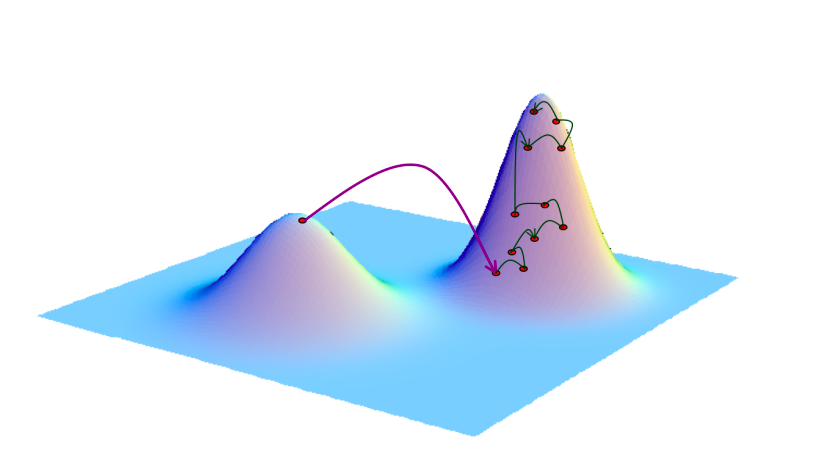
\includegraphics[width=15cm]{MCMC_figs/dram_t1d_final/multimodal_search.png}
    \caption{Graphical representation of how the DRAM can efficiently explore different maxima of the target distribution. Areas in purple tones indicate ares of higher probability parameter space, while areas in blue indicate areas of lower probability. This figure is adapted from Figure 3 of the reference \cite{trias2009delayed}.}
    \label{fig:globalmax}
\end{figure}
\par To compare the performace of the Metropolis and the DRAM MCMC methods on estimating the Lotka-Volterra model parameters, we first compare the sampling chains
\begin{figure}[H]
\begin{subfigure}{.5\textwidth}
  \centering
  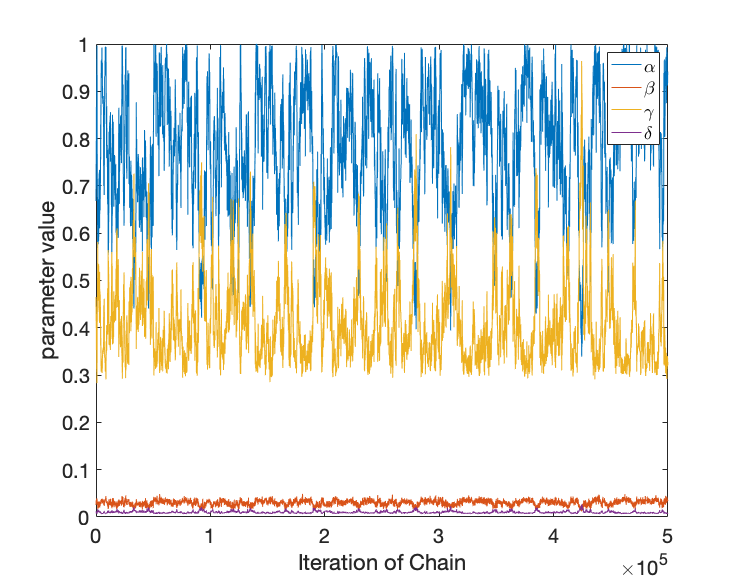
\includegraphics[width=1\linewidth]{MCMC_figs/met_lv_final/final_mh_chain.png}
  \caption{Metropolis MCMC sample chain.}
  \label{fig:11amcmcm}
\end{subfigure}
\begin{subfigure}{.5\textwidth}
  \centering
  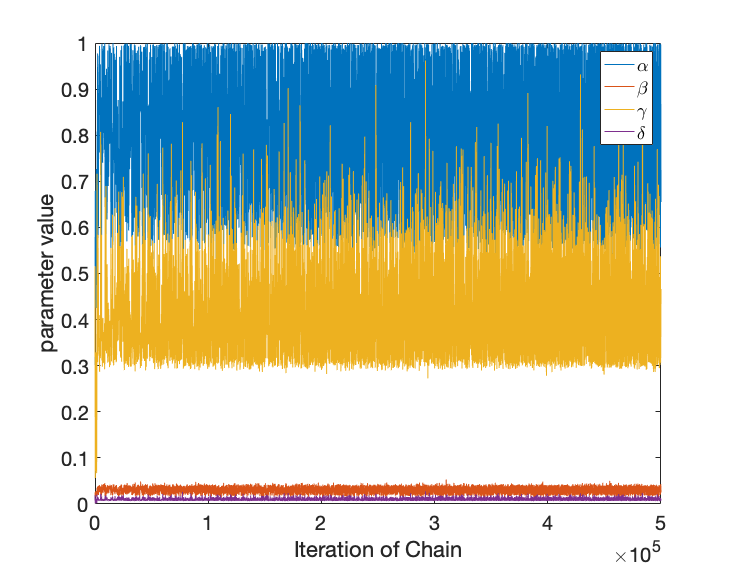
\includegraphics[width=1\linewidth]{MCMC_figs/met_lv_final/final_dram_chain.png}
  \caption{DRAM MCMC sample chain}
  \label{fig:11bmcmcm} 
\end{subfigure}
\caption{Comparing visual results of the sample chains from Metropolis and DRAM MCMC. The DRAM chain exhibits better mixing as it has the distinct ``fuzzy caterpillar" pattern.}
\label{fig:11mcmc}
\end{figure}
As we mentioned earlier, the ideal chain would be ``fuzzy catepillar-like" and we see this illustrated well in the DRAM algorithm, Figure \ref{fig:11bmcmcm}. It seems that the Metropolis chain has not done as good a job of sampling the parameter space, Figure \ref{fig:11amcmcm}. This so far this suggests that the DRAM is doing a better job of exploring the sampling space.
\par Next let's compare the computed results of these chains
%dram: .2406
% 0.0242
\begin{table}[H]
\centering
        \begin{tabular}{c | c | c c | c || c}
            \cline{1-6}
           \textbf{Parameter} & \textbf{Algorithm} &  \textbf{Mean} & \textbf{Std} &  \textbf{Geweke p-values} & \textbf{Chain Acceptance Rate}\\ 
            \cline{1-6}
            
            \multirow{2}{*}{\textbf{$\alpha$}} & Met & 0.779 & 0.134 & 0.895 & \multirow{4}{*}{\textbf{Met: 0.0242}}\\
            & DRAM & 0.787 & 0.139 & 0.983 & \\\cline{1-5}
            \multirow{2}{*}{\textbf{$\beta$}} & Met & 0.0301 & 5.40e-03 & 0.906 \\
            & DRAM & 0.030 & 5.58e-03 & 0.989 & \\ \cline{1-5}
            \multirow{2}{*}{\textbf{$\gamma$}} & Met & 0.412 & 0.0871 & 0.905 & \multirow{4}{*}{\textbf{DRAM: 0.2406}}\\
            & DRAM & 0.407 & 0.0908 & 0.931\\ \cline{1-5}
            \multirow{2}{*}{\textbf{$\delta$}} & Met & 9.95e-03 & 2.30e-03 & 0.902\\
            & DRAM & 9.83e-03 & 2.39e-03 & 0.933
             \\\hline
             \hline
        \end{tabular}
    \caption{Comparison of the results of the Metropolis and DRAM MCMC chains per parameter. There do not appear to be any significant differences in parameter values between the two algorithms. The only significant difference between the Geweke p-values occurs for $\alpha$. The DRAM appears to reach a better convergence than the Metropolis algorithm. The DRAM chain acceptance rate is significantly closer to the indicative threshold of 25\%. We do not yet discern any significant differences between the performances of each chain.}
    \label{tab:3mcmc}
\end{table}


We do not see any significant differences in individual parameter values between the two algorithms. While both p-values for $\alpha$ indicate that we fail to reject that the chain has converged, we note the difference as a possible explanation for the visual difference between $\alpha$'s PDFS. In Figure \ref{fig:4mcmc} we saw a lack of smoothness, while in Figure \ref{fig:9mcmc} we did see a more smooth distribution. Lastly we note the difference in chain acceptance rates. While not a perfect indicator of chain performance, we note that the DRAM algorithm's chain acceptance rate is much closer to the general threshold of 25\% acceptance. 

\par Next, we visually compare the PDFs of each parameter from both MCMC algorithms.
\begin{figure}[H]
    \centering
    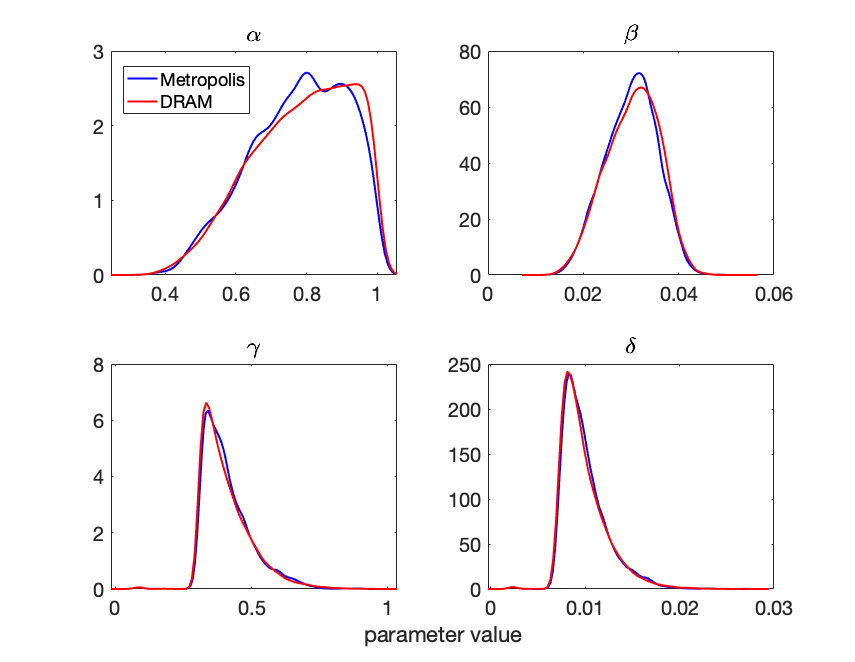
\includegraphics[width=15cm]{MCMC_figs/met_lv_final/overlaid_param_pdfs.png}
    \caption{Parameter posterior density distributions from both the Metropolis and DRAM parameterizations plotted together. We can see that the distributions are generally very similar as was evidenced in Table \ref{tab:3mcmc}. Visually, the distributions for $\alpha$ and $\gamma$ appear to differ the most.}
    \label{fig:overlayPDF_met}
\end{figure}
We can see that between the two algorithms, all of the parameters have very similar distribution shapes. In particular, the PDFS of $\gamma$ and $\delta$ are very similar. On the other hand, $\alpha$ and $\beta$ appear to differ more. Most notably, the Metropolis PDF for $\alpha$ is less smooth than that of the DRAM and appears to have 2 smaller peaks. Earlier, we discussed this visual discrepancy in terms of the statistical analysis of convergence with the Geweke p-values. Indeed, here we can see that as the $\alpha$ p-value from the Metropolis was the smallest, the corresponding PDF is the least smooth. Despite these few discrepancies, we believe that both the Metropolis and DRAM algorithms are producing comparable distributions for all the parameters.
\par Below we do a second visual assessment of the difference between means of parameters between distributions.
\begin{figure}[H]
\begin{subfigure}{.5\textwidth}
  \centering
  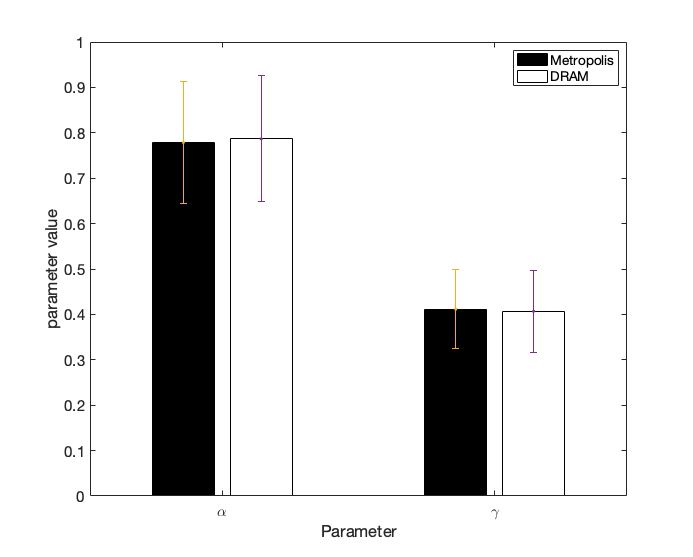
\includegraphics[width=1\linewidth]{MCMC_figs/met_lv_final/mh_dram_paramComp1.png}
  \caption{Comparison of means for $\alpha$ (left) and $\gamma$ (right).}
  \label{fig:12amcmcm}
\end{subfigure}
\begin{subfigure}{.5\textwidth}
  \centering
  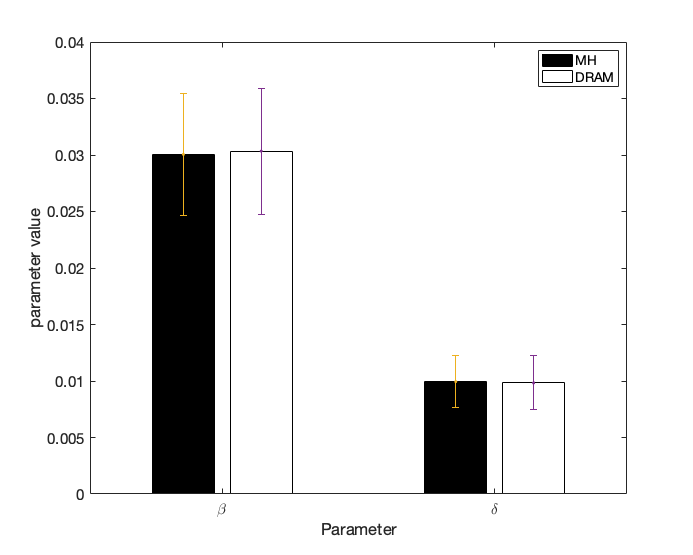
\includegraphics[width=1\linewidth]{MCMC_figs/met_lv_final/mh_dram_paramComp2.png}
  \caption{Comparison of means for $\beta$ (left) and $\delta$ (right).}
  \label{fig:12bmcmcm} 
\end{subfigure}
\caption{Comparing parameter means between the Metropolis and DRAM algorithms. Error bars were calculated using 1 standard deviation from Table \ref{tab:3mcmc}. We can see that no parameter mean values are significantly different.}
\label{fig:12mcmc}
\end{figure}
From both Table \ref{tab:3mcmc} and Figure \ref{fig:12mcmc}, we see that both algorithms are producing very similar values for each of the parameters. Figure \ref{fig:12mcmc} shows us that the means produced by each algorithm are not significantly different. This tells us both algorithms are finding the same parameter ranges in the parameter space. In order to truly compare the the performance of these two algorithms, we can compare the convergences and chain acceptance rates. While for both algorithms, we consider the chains to have converged for all parameters (Geweke $\geq 0.7$), we see that overall, the DRAM algorithm has Geweke values closer to 1. We do not have a definite reasoning for why there would be higher Geweke values for DRAM might be greater than those of the Metropolis MCMC, but we speculate that it is perhaps due to the overall sampling shapes that we saw in Figure \ref{fig:11mcmc}. With a more uniformly incremented selection of parameters, as in the DRAM algorithm, when we take the means of the first 10$\%$ and last $50\%$ of the chain, they are more likely to be very similar. On the other hand, in the Metropolis algorithm, since there is less uniformity when choosing the increments between samples, these same means are less likely to be so similar. And we can see this reflected in the difference in Geweke values. Lastly, we briefly compare the chain acceptance rates. As we mentioned before, a very general threshold for acceptance rates is around $25\%$ and is an indicator that the chain has converged and performed well. We more formally validate chain performance using the Geweke diagnostics that both chains have converged, but since the chain acceptance rate for Metropolis MCMC is significantly less than 0.25, we wonder if our algorithm is not performing as well as the DRAM algorithm.
\par We note that our statement of better performance with the DRAM algorithm is only in the context of our tutorial - that is with our specific model, burn-in period, total number of samples, likelihood functions, etc. Although we have not explored it here, increasing the number samples or tuning other parts of the Metropolis algorithm might in fact produce better results than the DRAM algorithm. The purpose of these tutorials is to help the user become more familiar with these two algorithms so that he or she can make an informed decision in choosing which algorithm to use.
\par Finally, we compare the predicted populations for hare and lynx given by parameter estimations from the Metropolis and DRAM MCMC method.
\begin{figure}[H]
    \centering
    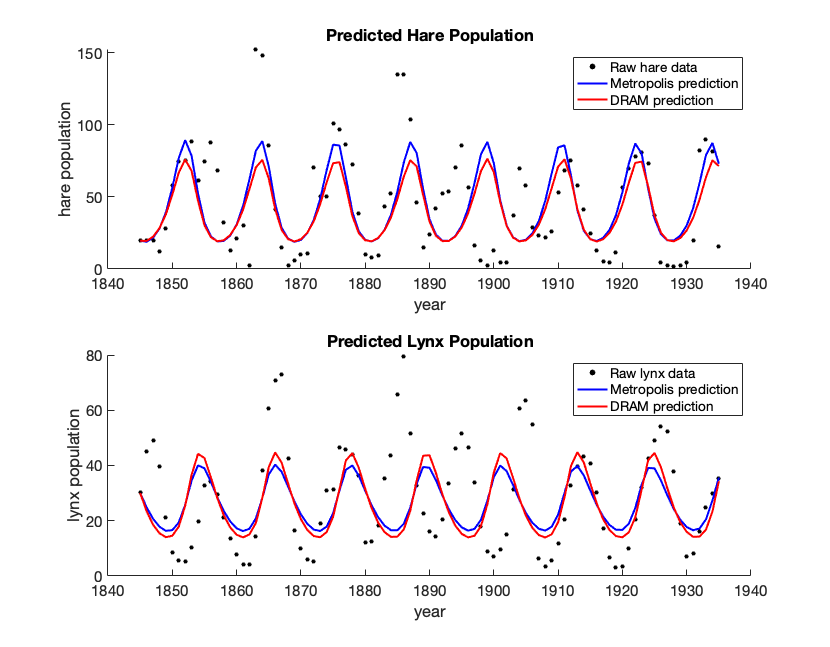
\includegraphics[width=15cm]{MCMC_figs/dram_mh_meanpredComp.png}
    \caption{Comparing mean predictions of the Metropolis and DRAM MCMC methods. Overlaid in black is the original raw hare and lynx data. Both predictions appear to capture the end behavior of the raw data, but fail to capture the starting behavior. It is difficult to visually determine which algorithm produces a better prediction.}
    \label{fig:13mcmc}
\end{figure}
While our predictions do not perfectly capture the original data, the period of each prediction is very similar to that of the original data. However, we do note some differences between the original data and each algorithm's prediction. In the lynx populations, both algorithms predict an initial decrease in population while the raw data has an increase instead. Both algorithms have a consistent period and amplitude while the raw data for both hare and lynx populations does not, thus both predictions miss a significant amount of the raw data from 1840 to around 1900. However, when the raw data becomes more consistent, around 1910 to 1940, with less variation in the period and amplitude, both predictions are able to capture these data points better. It is interesting to note that for the hare population, the Metropolis function predicts a periodic function with a greater amplitude than the DRAM algorithm and vice versa for the lynx population. But in both population predictions, they have very similar periods. 
\par While we have thus far presented several techniques for assessing algorithm performance, visual assessment of trace plots, the Geweke diagnostic, and chain acceptance rate, we base our evaluation more heavily on determining whether our algorithm has produced a prediction that captures the raw data well. In Figure \ref{fig:13mcmc}, we believe that both our algorithms have satisfactorily captured the data. We will quantify the performance more formally using root mean squared error in Table \ref{tab:4mcmc}.
\begin{table}[H]
\centering
        \begin{tabular}{c | c c}
            \cline{1-3}
            \textbf{MCMC Algorithm}  &\textbf{Hare} & \textbf{Lynx}\\
            \hline
            Metropolis & 18.16 & 31.30\\
            DRAM & 18.03 & 31.66
             \\\hline
            \hline
        \end{tabular}
    \caption{Formal comparison of the Metropolis and DRAM MCMC methods on the Lotka-Volterra system using root mean squared error (RMSE). Based on RMSE scores, there is no significant difference between the two predictions. We conclude that both the Metropolis and DRAM parameter estimations produce satisfactory populatin predictions that capture the raw data well.}
    \label{tab:4mcmc}
\end{table}
Figure \ref{fig:13mcmc} showed us that the two algorithms performed very similarly and Table \ref{tab:4mcmc} confirms this. A perfect fit of the data by the prediction would produced an RMSE score of 0. While it is difficult to formally determine an RMSE threshold for prediction performance, we consider the scores in Table \ref{tab:4mcmc} to indicate that the data was captured fairly well. In general, we would say that an RMSE score of $>$100 would indicate poor performance. While DRAM appears to perform better on the hare population prediction and the Metropolis appears to perform better on the lynx population prediction, there is no significant difference between the RMSE scores. Both Figure \ref{fig:13mcmc} and Table \ref{tab:4mcmc} suggest that both the DRAM and Metropolis MCMC algorithms can perform comparably well on this Lotka-Volterra system.
\par Perhaps it is due to the simplicity of the Lotka-Volterra model and relatively low-dimensional parameter space, that we are able to produce fairly similar predictions. However, taking note of the discrepancies between the two algorithms that we discussed early, we might assume that as a model becomes more complex and the parameter space increases exponentially (recall the curse of dimensionality), these differences may also increase. Thus, as we will parameterize the Type 1 Diabetes model in the next section, we choose to do so with the DRAM MCMC algorithm. So far this algorithm has demonstrated sufficient chain sampling (Figure \ref{fig:11bmcmcm}), convergence (Table \ref{tab:3mcmc}), and smooth distributions (Figure \ref{fig:9mcmc}).

\subsection{Parameterizing the Type 1 Diabetes Model with DRAM} \label{Parameterizing_T1D_DRAM}
We preface this section by saying that the implementation of the DRAM algorithm for the Type 1 Diabetes model is still in the process of being fine-tuned and improved. Therefore, we advise the reader to read our code and comments thoroughly and to analyze our results with some caution and skepticism.
\par We consider 10 parameters in this model, as for reasons discussed in \textbf{Sections \ref{section:NotableParameterSubset} and \ref{section:NumParamsMCMC}}, we could not parameterize all 53 parameters in the T1D ODE system. Thus we carefully chose parameters that we determined had the greatest impact on the system. The UKF algorithm found 7 parameters that seemed to vary more greatly than the others. We know from our advisors and the Shtylla et al. 2019 paper, that the eta parameters, $\alpha_{\eta}$, $\beta_{\eta}$, and $\eta$ had a great impact on diabetes onset time. Lastly, we ran our algorithm on the model for NOD mice with the apoptotic $\beta$-cell wave on. We choose these settings because all the mice in the Li et al study developed diabetes. A NOD mouse with an apoptotic $\beta$-cell wave are the biologically modelled conditions under which diabetes will occur \cite{shtylla2019mathematical}. 
\par Similar to Lotka-Volterra parameterization, we assume a Gaussian likelihood function in log base e. We implement a sum of squares function for our likelihood function (recall Step 3 of the DRAM algorithm) and so working with log values prevents our sums from increasing exponentially. Thus, the user determines a sum of squares between the model given parameter values and the original data. This sum of squares is then used to construct the acceptance criterion
\begin{equation} \label{eq:19mcmc}
lnP(D|\theta, M) = \sum_{k=1}^{N}lnP(y_k|x_k,\theta,M) = \sum_{k=1}^N SS_\theta 
\end{equation}
 We also again adopt a log-uniform prior
\begin{equation} \label{eq:20mcmc}
lnP(\theta|M) = 0
\end{equation}
The proposal distribution is determined for us in the MATLAB function \texttt{mcmcrun} using a covariance matrix. The acceptance criteria according to the \texttt{mcmcstat} library is defined as
\begin{equation} \label{eq:21mcmc}
\alpha = min(1, e^{ \lbrack {-0.5(\frac{\sum (SS_{\theta^*}-SS_{\theta^{k-1}})}{\sigma^2} + prior^*-prior^{k-1})} \rbrack}) 
\end{equation}
and thus with our assumptions simplifies to 
\begin{equation} \label{eq:22mcmc}
\alpha = min(1, e^{[ {-0.5(\frac{\sum (SS_{\theta^*}-SS_{\theta^{k-1}})}{\sigma^2}]}})
\end{equation}
Lastly, we initialize starting values and ranges for our parameters.
With all of these assumptions and initializations, we can run the DRAM MCMC algorithm and produce PDFs for each of our parameters.
\par We ran the DRAM algorithm on 4 sets of data. The first is the average acute Li mouse data that was described in the Section Problem Set Up. For comparison with this data set and UKF predictions, we also ran our algorithm on a single mouse's data set. Mouse 6 is an example of an acute mouse that we chose because of its relatively large number of data points. Lastly, we ran the algorithm using Mouse 3 and 11 (individual runs). We had visually determined that these two mice had significantly different diabetes onset times and we were interested in exploring how the algorithm's prediction would shift with this shift in onset time. 
\par In the following sections, we analyze the results of running the DRAM algorithm on the averaged data and Mouse 6 data using techniques we developed while parameterizing the Lotka-Volterra system.
\subsubsection{Parameterizing with Averaged Data}
\paragraph{Analyzing the chain}
Before jumping straight into using the results of the DRAM algorithm, we want to look at our chain for information about the algorithm's performance. We begin by looking at the trace plots of the chain for each of the parameters. We performed a burn-in period of 1,000 samples, but we only present the trace plots of the post-burn-in chain.
\begin{figure}[H]
    \centering
    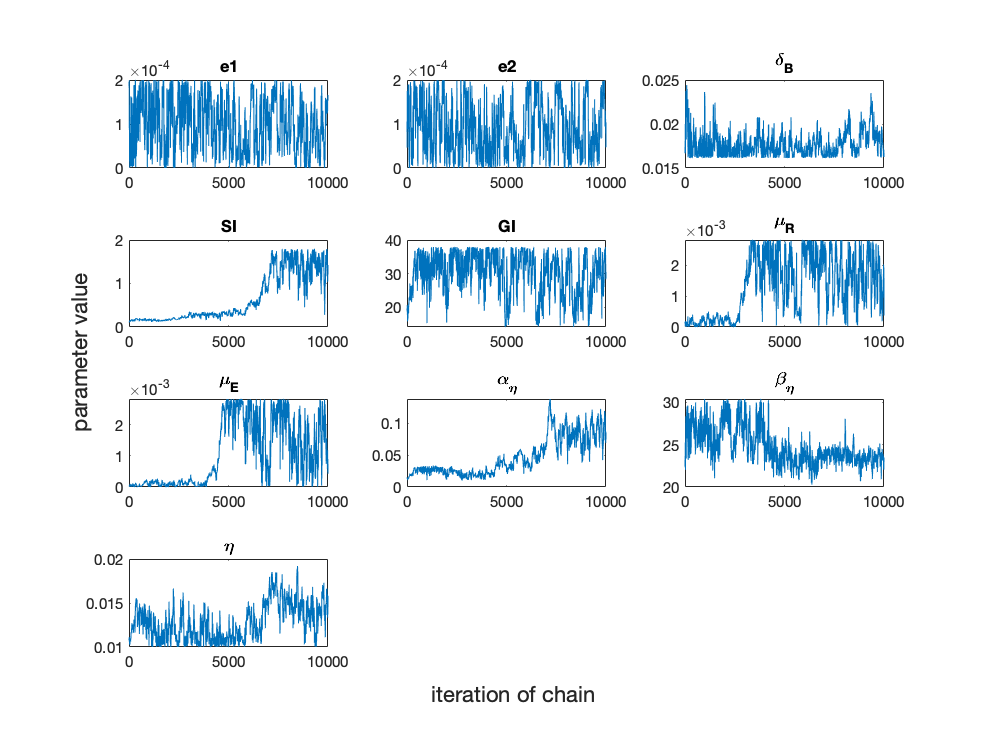
\includegraphics[width=15cm]{MCMC_figs/dram_t1d_final/final_dram_avg_traceplot.png}
    \caption{Trace plots of the sampling chain (10,000 samples) for the DRAM MCMC parameterization of the Type 1 Diabetes model on averaged Li data. Chains for each parameter are plotted separately. There are examples of good and bad chain mixing. e1 and e2 exhibit good chain mixing while $\alpha_\eta$ has poor mixing. Poor mixing is indicative of a lack of convergence.}
    \label{fig:14mcmc}
\end{figure}
We have chosen to plot each trace plot separately because the scale of the value ranges for each parameter varies greatly. Overall, there seems to be ``good" and ``bad" mixing. As we learned from looking at the chain trace plots of the Lotka-Volterra model, we would like to see a dense plot. By eye, we can see some examples of good mixing in the plots for e1, e2, and GI. Plots for $\delta_B$, $\beta_{\eta}$, and $\eta$ show moderately good mixing. The trace plots for SI, $\mu_R$, $\mu_E$, and $\alpha_{\eta}$ show a shift in parameter mean value as their mixing pattern appears to shift after a certain number of samples. We have already taken a burn-in period, but it may be that these final 4 parameters needed more time to converge. We turn to formal techniques of determining convergence to investigate the effects of the bad chain mixing.
                            
\begin{table}[H]
\centering
        \begin{tabular}{c c |c c | c c||c}
            \hline
            \textbf{Parameter} & \textbf{Initial Value} & \textbf{Mean} &  \textbf{Std} & \textbf{Geweke} & \textbf{ p-value} &\textbf{Chain Acceptance Rate}\\ 
            \cline{1-7}
            e1 & 1.0e-08 & 9.9199e-05 & 5.6117e-05 & 0.4099 &  0.68184 & \multirow{10}{*}{0.43370} \\
            e2 & 1.0e-08 & 9.2374e-05 & 5.9001e-05 & 0.2947 & 0.76824\\
            $\delta_B$ & 0.0167 & 0.017692 &  0.001341 & 0.0248 & 0.98022\\
            SI & 0.72 & 0.6345 & 0.5506  & -1.8522 & 0.063996\\
            GI & 141.4214 & 30.125 & 6.02 & 0.0436 & 0.96526\\
            $\mu_R$ & 2.0e-06 & 0.0013304 & 0.00095325 & -2.1923 & 0.028361\\
            $\mu_E$ & 2.0e-06 & 0.0010473 &  0.0010099 & -2.3090 & 0.020945\\
            $\alpha_{\eta}$ & 0.0100 & 0.04688 &  0.029704 & -1.4409 & 0.14961\\
            $\beta_{\eta}$ & 22 &  24.723 & 2.0772 & 0.2178 & 0.82762\\
            $\eta$ & 0.100 & 0.012852 &  0.0020148 & -0.1080 & 0.914
             \\\hline
                          \hline
        \end{tabular}
    \caption{Table listing results of the DRAM chain on the Type 1 Diabetes model for averaged Li data. Parameter means, standard deviations, and convergence diagnostics (Geweke) are calculated. Based on the Geweke p-values, chain has not converged for all parameters. Using a p-value of 0.05 to indicate rejection of the null hypothesis, the parameters $\mu_R$ and $\mu_E$ have statistically not converged. Parameters SI and $\alpha_\eta$ have very low p-values close to 0.05 so we are less confident in their mean values. The chain acceptance rate, while not 25\%, indicates that the algorithm is searching and accepting or rejecting candidates efficiently.}
    \label{tab:5mcmc} 
\end{table}
Unlike our Lotka-Volterra model, the chain has not converged for all of our parameters. Notably, parameters $\mu_R$ and $\mu_E$ have Geweke p-values of $< 0.05$ and thus we say that we reject the null hypothesis that the chain has converged for these parameters. Using the p-value threshold of 0.05, we say that parameters SI and $\alpha_\eta$ have converged, however their p-values are relatively low and close to 0.05 ($\sim 0.064$ and $\sim 0.15$ respectively), so we are more skeptical of their means. For the remaining parameters, e1, e2, $\delta_B$, GI, $\beta_\eta$, and $\eta$, we are confident in their mean values as based on their p-values, we fail to reject the hypothesis that the chain has converged. We note that Geweke values and their p-values may improve if we allow the algorithm to take more samples. When estimating parameters for the Lotka-Volterra model, we implemented a burn-in period of 10,000 samples and a full sampling chain of 500,000 samples. We did not do the same for the T1D model parameter estimation as the computation time increased exponentially. With a 1,000 sample burn-in period and 10,000 sample chain, our algorithm takes around 1 hour to run on a standard MacBook Air. In order to increase computational efficiency and run the DRAM algorithm for more iterations we recommend the use of a computer cluster.
\par When analyzing the chain acceptance rate of the Lotka-Volterra model, we cited literature that used an acceptance rate of around 25\% to indicate an efficient, convergent, well-performing chain \cite{convergence}. However, other authors argue that for increasingly large and complex systems, this threshold acceptance rate should also increase. In addition, they also point out that in large systems, such as the type 1 diabetes model, it is not feasible to prescribe a universal acceptance rate threshold because the interactions of the model's states and parameters will be specific to that model thereby affecting the overall acceptance rate \cite{converge_threshold}. A more in-depth investigation into the role of chain acceptance rates for large systems will be needed. For now, we are satisfied that the acceptance rate is at least significantly less than 100\%. Given these results good and bad, we are satisfied with the performance of our algorithm. We will discuss more about how we might want to determine good performance in future uses in the Discussion section.
\par Next we visualize the parameter posterior distributions.
\begin{figure}[H]
    \centering
    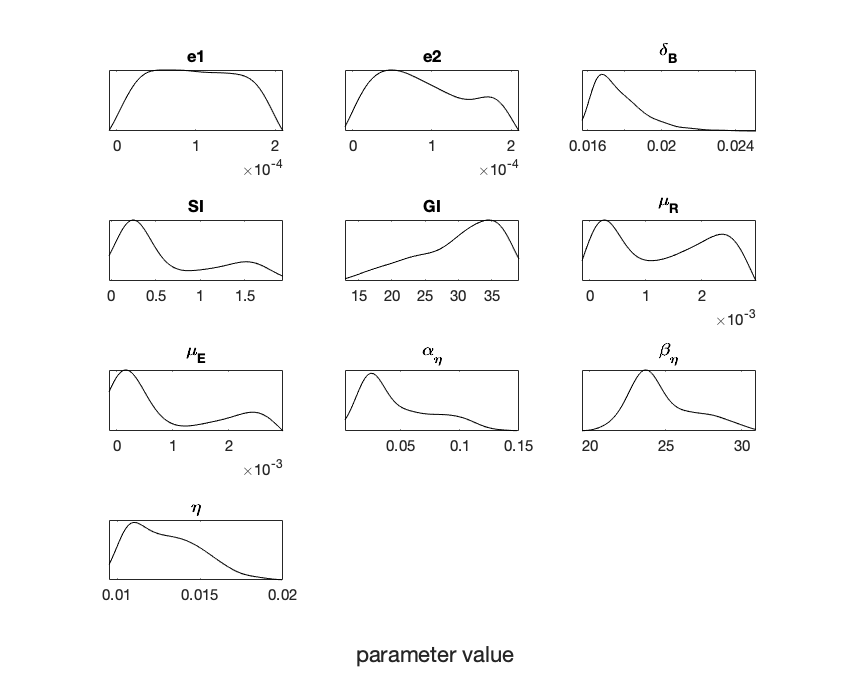
\includegraphics[width=15cm]{MCMC_figs/dram_t1d_final/jul10_avg_run1(noIC)_acute_NOD_waveOn_lietal_den.png}
    \caption{DRAM parameter distributions for 14 Type 1 Diabetes parameters for averaged Li data. Some parameters exhibit bimodal distributions. Specifically, $\mu_R$ and $\mu_E$ appear to have bimodal distributions. Recall from Table \ref{tab:5mcmc} that these parameters had very low Geweke values, this indicates that algorithm was not able to determine a global maximum for each parameter as is apparent in their distributions.}
    \label{fig:15mcmc}
\end{figure}
It is not useful for us to try to formally classify these distributions however, we can see some familiar shapes. Parameters $\delta_B$, $\alpha_eta$, and $\beta_{\eta}$ appear log-normal-ish. Others like e1 and e2 appear almost uniform. Lastly, we make note of the parameters whose distributions seem to be bimodal: SI, $\mu_R$, and $\mu_E$ are the most pronounced, but an argument could be made for the bimodal pattern in some of the other parameters. It is also important to note that the chain had not converged for both $\mu_R$ and $\mu_E$ according to their p-values in Table \ref{tab:5mcmc} and SI had a p-value of $\sim 0.064$, very close to the 0.05 threshold. The lack of convergence that we saw statistically is corroborated with these bi-modal distributions. We hypothesize that the algorithm was not able to determine a global maximum for SI, $\mu_R$, and $\mu_E$ and thus sampled in two ranges resulting in the bi-modal distribution and lack of convergence. However, it is important to remember that some parameters may not have a global maximum and instead have multiple local maxima, that is they may have more than one optimal range of values (it will likely depend on a parameter's individual interaction with another parameter). Altogether, these distributions appear relatively smooth, which unfortunately does not give us any other clues for the lack of convergence that we saw in Table \ref{tab:5mcmc}.
\paragraph{Working with the distributions}
Now that we have an understanding of the performance of our chain, we can explore the predicted results. We first look at model prediction that uses DRAM's mean parameter values.
\begin{figure}[H]
\centering
\begin{subfigure}{.7\textwidth}
    \centering
    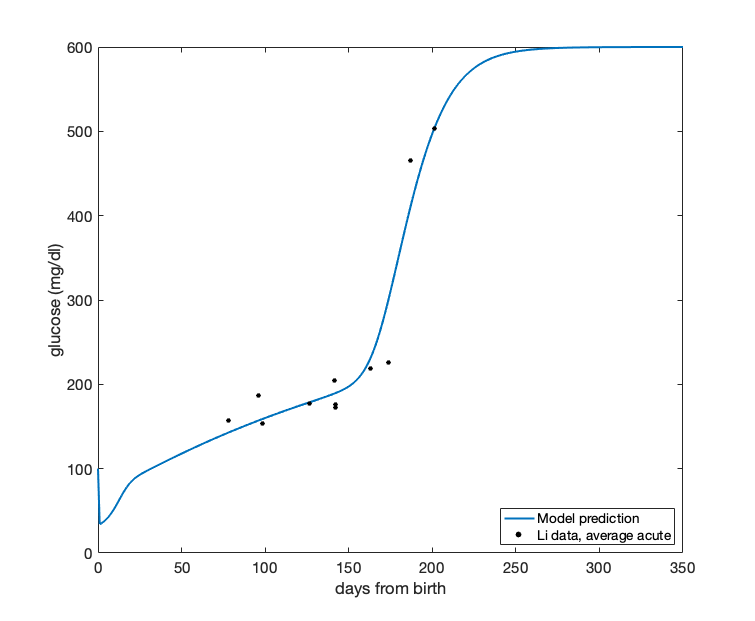
\includegraphics[width=1\linewidth]{MCMC_figs/dram_t1d_final/jul10_avg_run1(noIC)_acute_NOD_waveOn_lietal_meanpred.png}
    \caption{Predicted Glucose model plotted using mean DRAM parameter values.}
    \label{fig:17amcmc}
\end{subfigure}
\begin{subfigure}{.7\textwidth}
    \centering
    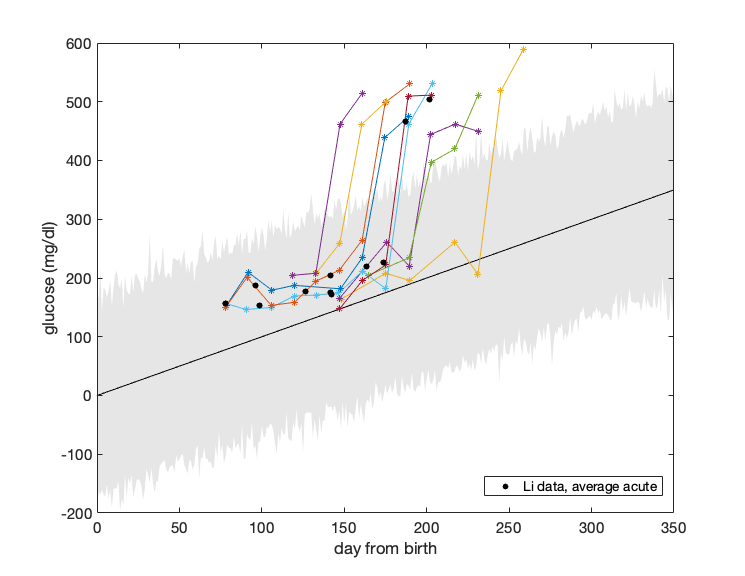
\includegraphics[width=1\linewidth]{MCMC_figs/dram_t1d_final/95_CI_avg.png}
    \caption{Predicted glucose model with $95\%$ probability range plotted with averaged acute data and the 9 acute Li et al. mice.}
    \label{fig:17bmcmc}
\end{subfigure}
\caption{Plotting glucose predictions. In 23(a), the averaged acute Li data is plotted over the prediction. The prediction appears to capture the original data fairly well. We see the characteristic acute mouse slow steady increase and then spike of glucose indicating diabetes onset. In 23(b), the prediction does not appear to capture the original data well as not all the data points are captured within the $95\%$ probability range. It is unclear to us why these two predictions produce such different results.}
\label{fig:17mcmc}
\end{figure}
In Figure \ref{fig:17bmcmc}, we present a figure analogous to the Lotka-Volterra predictions in Figures \ref{fig:5mcmc} and \ref{fig:10mcmc}. In addition to the 95$\%$ prediction range, we plot the original 9 acute mice data and the averaged acute data. Although a majority of the points are captured within the $95\%$ probability range, we are unsure why the overall trend of these predictions is linear. It is important to note that we did not write the code that plots Figure \ref{fig:17bmcmc}, so it is difficult for us to tune the plot. The reason that we believe that there are plotting issues that figures is that when we plot Figure \ref{fig:17amcmc}, the prediction is actually fairly good. This is something to be investigated in the future.). In Figure \ref{fig:17mcmc}, we only plot one prediction of the glucose state using the DRAM mean parameter values. From this figure, it seems that this prediction is capturing the original data quite well and we are satisfied with the overall trend of the prediction. 

\subsubsection{Parameterizing with Mouse 6 Data}
We chose to run the DRAM algorithm on a single mouse because we want to see the results using only raw data. Recall that in the averaged data, we had to make some assumptions about the overall time frame of our data. With mouse 6 data, we can avoid over-generalization and making assumptions. 
\paragraph{Analyzing the chain}
We begin by looking at the trace plots of the chain for each of the parameters. We performed a burn-in period of 1,000 samples, but we only present the trace plots of the post-burn-in chain.
\begin{figure}[H]
    \centering
    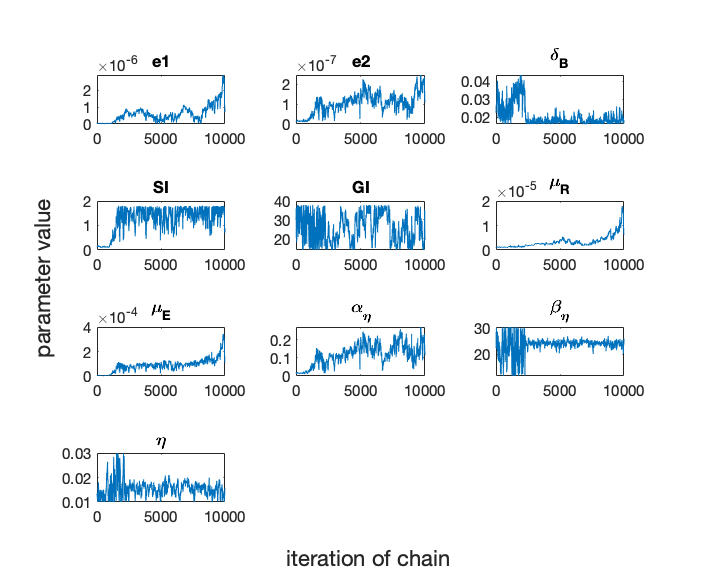
\includegraphics[width=15cm]{MCMC_figs/dram_t1d_final/final_dram_mouse6_traceplots.png}
    \caption{Trace plots of the sampling chain (10,000 samples) for the DRAM MCMC parameterization of the Type 1 Diabetes model on mouse 6 only. Chains for each parameter are plotted separately. We see a mixture of good and poor chain mixing. GI exhibits good mixing while $\mu_R$ and $\mu_E$ exhibit bad mixing. This indicates that chain has not converged for parameters with poor mixing.}
    \label{fig:18mcmc}
\end{figure}
Immediately we see that there is an overall lack of good mixing. Parameter GI seems to be the closest to having good mixing. It is interesting to see now that we can determine some of the parameters that will not have converged. Parameters $\delta_B$, $\beta_{\eta}$, and $\eta$ have pretty dramatic shifts in means during the 10,000 iterations. Recalling the definition of Geweke's diagnostic, these 3 parameters are unlikely to have similar means for the first 10\% and last 50\% of their chain, thus we know that they have not converged. However, these convergences are likely better, in comparison to parameters whose trace plots look like e1, e2, $\mu_R$, $\mu_E$, and $\alpha_{\eta}$. These barely look like classic chain trace plots and their means are almost constantly changing. We turn to formal techniques of determining convergence to investigate the effects of the poor chain mixing.
\begin{table}[H]
\centering
        \begin{tabular}{c c|c c | c c ||c}
            \hline
            \textbf{Parameter} & \textbf{Initial Value} & \textbf{Mean} &  \textbf{Std} & \textbf{Geweke} & \textbf{p-value} &\textbf{Chain Acceptance Rate}\\ 
            \cline{1-7}
            e1 & 1.0e-08 & 5.9625e-07 & 4.8352e-07 & -2.2691 & 0.023261 & \multirow{10}{*}{0.541} \\
            e2 & 1.0e-08 & 1.0391e-07 &  5.029e-08 & -2.2122 & 0.026956\\
            $\delta_B$ & 0.0167 & 0.020498 &  0.0057686 &  0.5394 & 0.58958\\
            SI & 0.72 &  1.2582   &  0.50705  & -2.2012 & 0.027721\\
            GI & 141.4214 &  25.949 &  7.0361 & 0.1279 & 0.89823\\
            $\mu_R$ & 2.0e-06 & 3.3264e-06 & 2.5351e-06 & -1.8527 & 0.063928\\
            $\mu_E$ & 2.0e-06 &  8.8867e-05 & 5.2077e-05 & -2.4567 & 0.014021\\
            $\alpha_{\eta}$ & 0.0100 & 0.11996 & 0.057717 & -2.1727 & 0.029801\\
            $\beta_{\eta}$ & 22 &  23.507 & 2.8037 & -0.1665 & 0.86778\\
            $\eta$ & 0.0100 & 0.015418 &  0.0031396 & -0.2313 & 0.81708
             \\\hline
                          \hline
        \end{tabular}
    \caption{Table listing results of the DRAM chain on the Type 1 Diabetes model for mouse 6 only. Parameter means, standard deviations, the convergence diagnostic (Geweke), and Geweke p-values are calculated. Based on the Geweke p-values, the chain has not converged for all parameters. In particular, parameters e1, e2, SI,  $\mu_E$, and $\alpha_\eta$ have p-values $< 0.05$ thus we reject the hypothesis that the chain has converged for these parameters. The chain acceptance rate seems to be a reasonable value as it is not significantly larger than 50\% and is much less than 100\%.}
    \label{tab:6mcmc}
\end{table}
Compared with the parameters from the DRAM parameter estimation using the averaged data, in Table \ref{tab:6mcmc} we have significantly less convergence (Table \ref{tab:5mcmc}). Parameters e1, e2, SI,  $\mu_E$, and $\alpha_\eta$ all have p-values $< 0.05$ and thus we must reject the null hypothesis that the chain has converged for these parameters. The parameter $\mu_R$ has a p-value of $\sim 0.064$ which is close to our threshold of 0.05, thus we are less confident in the accuracy of the mean of this parameter. For the remaining parameters, $\delta_B$, GI, $\beta_\eta$, and $\eta$, we fail to reject our null hypothesis and say that the chain has converged for these parameters. The chain acceptance rate does not give us much information regarding chain performance but for now, we are satisfied that the acceptance rate is not significantly larger than 50\% and is much less than 100\%. Thus, we believe our chain is giving a satisfactory parameterization. So far, the algorithm has not performed as well on the Mouse 6 data than on the averaged data.
\par Next we visualize the parameter posterior distributions.
\begin{figure}[H]
    \centering
    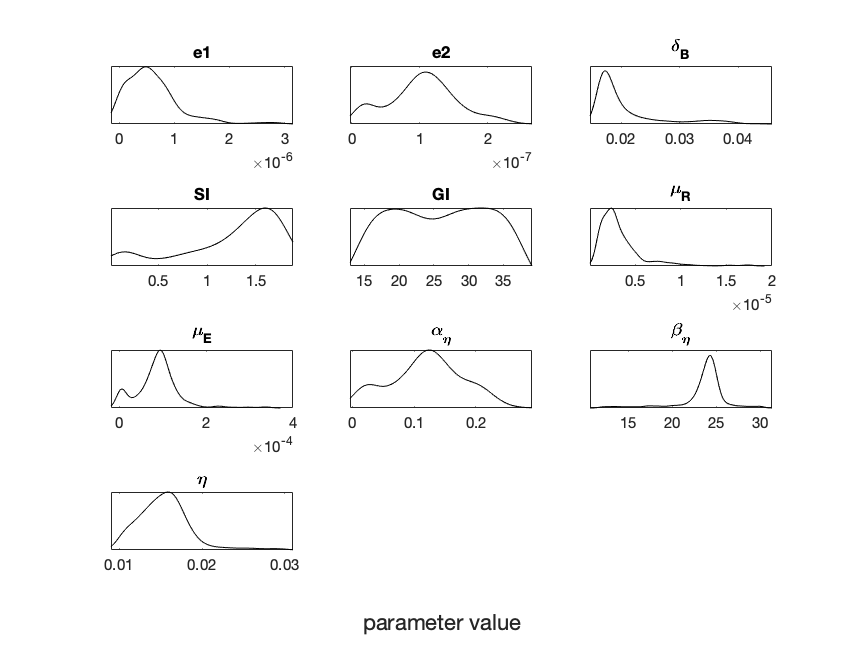
\includegraphics[width=15cm]{MCMC_figs/dram_t1d_final/jul10_mouse6_run1(noIC)_acute_NOD_waveOn_lietal_den.png}
    \caption{DRAM parameter distributions for 14 Type 1 Diabetes parameters for mouse 6. For some parameters, like $\mu_E$ and $\alpha_\eta$, the results of Table \ref{tab:6mcmc} are confirmed with bimodal distributions and lack of smoothness. We conclude that for some parameters, the algorithm was unable to determine the best range of values for that parameter.}
    \label{fig:19mcmc}
\end{figure}
Overall these distributions look drastically different than those in Figure \ref{fig:15mcmc} (we will do a more formal comparison of parameter means in a subsequent section). In looking at the distributions of the parameters for which the chain did not converge, e1, e2, SI,  $\mu_E$, and $\alpha_\eta$, we see that the distributions for e2, SI, $\mu_E$, and $\alpha_\eta$ appear to have some degree of bi-modal behavior. This is most pronounced in the PDFs of e2 and $\mu_E$. These bi-modal behaviors indicate and the lack of convergence that we saw in Table \ref{tab:6mcmc} indicates that the DRAM algorithm was struggling to determine a global maximum. It appears that it might have found two ranges of values with higher probability.
\paragraph{Working with the distributions}
Next we analyze the performance of the DRAM algorithm by assessing the fit of the glucose prediction that we can produce from the estimated parameter values.
\begin{figure}[H]
\centering
\begin{subfigure}{.7\textwidth}
    \centering
    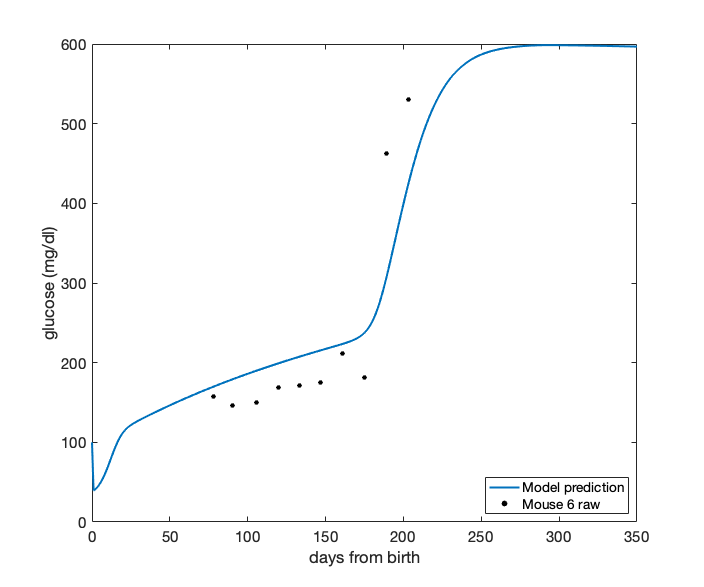
\includegraphics[width=1\linewidth]{MCMC_figs/dram_t1d_final/jul10_mouse6_run1(noIC)_acute_NOD_waveOn_lietal_meanpred.png}
    \caption{Predicted Glucose model plotted using mean DRAM parameter values. }
    \label{fig:mouse6amcmc}
\end{subfigure}
\begin{subfigure}{.7\textwidth}
    \centering
    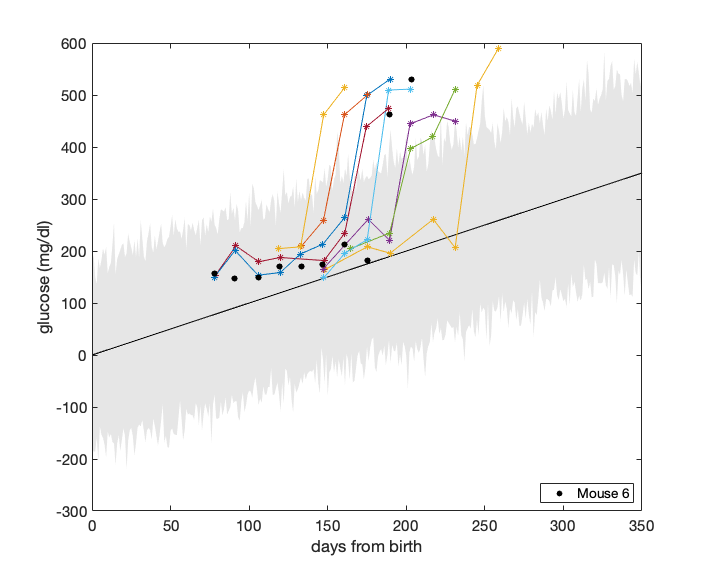
\includegraphics[width=1\linewidth]{MCMC_figs/dram_t1d_final/95_CI_mouse6.png}
    \caption{Predicted glucose model with $95\%$ probability range plotted with the 9 acute Li et al. mice.}
    \label{fig:mouse6bmcmc}
\end{subfigure}
\caption{Plotting glucose predictions from DRAM parameterization using Mouse 6 data. In 26(a), the Mouse 6 data is plotted over the prediction. Despite poor chain performance for some parameters, the prediction seems to capture the data fairly well. In 23(b), the prediction does not appear to capture the any of the individual mice well as not all the data points are captured within the $95\%$ probability range. It is unclear to us why these two predictions produce such different results.}
\label{fig:mouse6mcmc}
\end{figure}
We similar results from our parameterization using averaged data in Figure \ref{fig:mouse6bmcmc}. In addition to the 95$\%$ prediction range, we plot the original 9 acute mice data and the averaged acute data. Although a majority of the points are captured within the $95\%$ probability range, we are unsure why the overall trend of these predictions is linear. From Figure \ref{fig:mouse6amcmc}, it seems that our prediction is capturing the general trend of the original data, but it is not capturing the raw data as well as the prediction in Figure \ref{fig:17mcmc}. We are satisfied with the overall trend of the prediction, however, we are cautious in trusting the parameter values because a majority of our parameter did not show convergence (Table \ref{tab:6mcmc}). Nevertheless, we in the next section we compare the overall mean predictions and parameter values.
\subsubsection{Evaluating the DRAM Algorithm}
Our final step in assessing the DRAM algorithm is to evaluate and compare our parameter estimates from both the averaged acute and the Mouse 6 data sets. We do an evaluation both visually and formally using a mean-squared error score and finally, we compare the actual mean values of the parameters. 
\par Although we only present the full results from 2 different data sets used to parameterize the type 1 diabetes model, we have run the DRAM algorithm on 2 additional individual Mice, 3 and 11 in order to compare the role of the data set. We begin by comparing differences in parameters for which the chain has converged between parameterizations using the different data sets.
% 3: 0.8484    0.7691    0.9104    0.0710    0.4664               0.6179    0.1840    0.0242    0.8388    0.9860

% 11: 0.9249    0.7804    0.5049    0.0655    0.9074              0.0940    0.9985    0.0288    0.9937    0.7456
\begin{table}[H]
\centering
        \begin{tabular}{c|c c|c| c c}
            \hline
            \textbf{Parameter} & \textbf{Data Set} &  \textbf{Geweke p-value} & \textbf{Parameter} & \textbf{Data Set} &  \textbf{Geweke p-value} \\
            \cline{1-6}
            \multirow{4}{*}{e1} & Mouse 3 & 0.8484 & \multirow{4}{*}{$\mu_R$} & Mouse 3 & 0.6179\\
            & Mouse 6 & 0.023261 & & Mouse 6 & 0.063928\\
            & Mouse 11 & 0.9249 & & Mouse 11 & 0.0940\\
            & Averaged & 0.68184 & & Averaged & 0.028361 \\\hline
            \multirow{4}{*}{e2}  & Mouse 3 & 0.7691 & \multirow{4}{*}{$\mu_E$} & Mouse 3 & 0.1840\\
            & Mouse 6 & 0.026956 & & Mouse 6 & 0.014021\\
            & Mouse 11 & 0.7804 & & Mouse 11 & 0.9985\\
            & Averaged & 0.76824 & & Averaged & .020945\\\hline
            \multirow{4}{*}{$\delta_B$} & Mouse 3 & 0.9104 & \multirow{4}{*}{$\alpha_\eta$} & Mouse 3 & 0.0242\\
            & Mouse 6 & 0.58958 & & Mouse 6 & 0.029801\\
            & Mouse 11 & 0.5049 & & Mouse 11 & 0.0288\\
            & Averaged & 0.98022 & & Averaged & 0.14961 \\\hline
            \multirow{4}{*}{SI} & Mouse 3 & 0.0710 & \multirow{4}{*}{$\beta_\eta$} & Mouse 3 & 0.8388 \\
            & Mouse 6 & 0.027721  & & Mouse 6 & 0.86778\\
            & Mouse 11 & 0.0655 &&  Mouse 11 & 0.9937\\
            & Averaged & .063996 & & Averaged & 0.82762\\\hline
            \multirow{4}{*}{GI} & Mouse 3 & 0.4664  & \multirow{4}{*}{$\eta$} & Mouse 3 & 0.9860\\
            & Mouse 6 & 0.89823 & & Mouse 6 & 0.861708\\
            & Mouse 11 & 0.9074  & &Mouse 11 & 0.7456\\
            & Averaged & 0.96526 & &Averaged & 0.914\\\hline
             \hline
        \end{tabular}
    \caption{Table comparing the Geweke p-values for DRAM parameter estimates using 4 different data sets. Based on the p-values, the chain has converged for the parameters $\delta_B$, GI, $\beta_\eta$, and $\eta$ in all 4 parameterizations. For the rest of the parameters, there is a mixture of convergence and non-convergence between data sets.}
    \label{tab:pvalComp}
\end{table}
In Table \ref{tab:pvalComp} we compare the Geweke p-values from individual DRAM parameter estimations using 4 different data sets for each of the parameters. We note that we see only consistent convergence across data sets for the parameters $\delta_B$, GI, $\beta_\eta$, and $\eta$. All the other parameters have at least one data set for which the chain did not converge. For example, for the parameter e1, the chain has converged in the Mouse 3, Mouse 11, and Averaged data sets, yet it failed to converge for Mouse 6 as we see a p-value of $\sim 0.023$ which is $< 0.05$. While the p-values for e1 are fairly high for the Mouse 3, Mouse 11, and Averaged data sets (0.8484, 0.9249, and 0.68184 respectively), for other parameters like SI, the p-values are consistently low for all the data sets. While for SI, statistically we fail to reject the null hypothesis that the chain has converged in Mouse 3, Mouse 11, and the Averaged data sets, all 4 p-values are fairly close to the 0.05 threshold. Thus, we are less confident in the mean values of SI from each DRAM parameter estimation.
\begin{figure}[H]
    \centering
    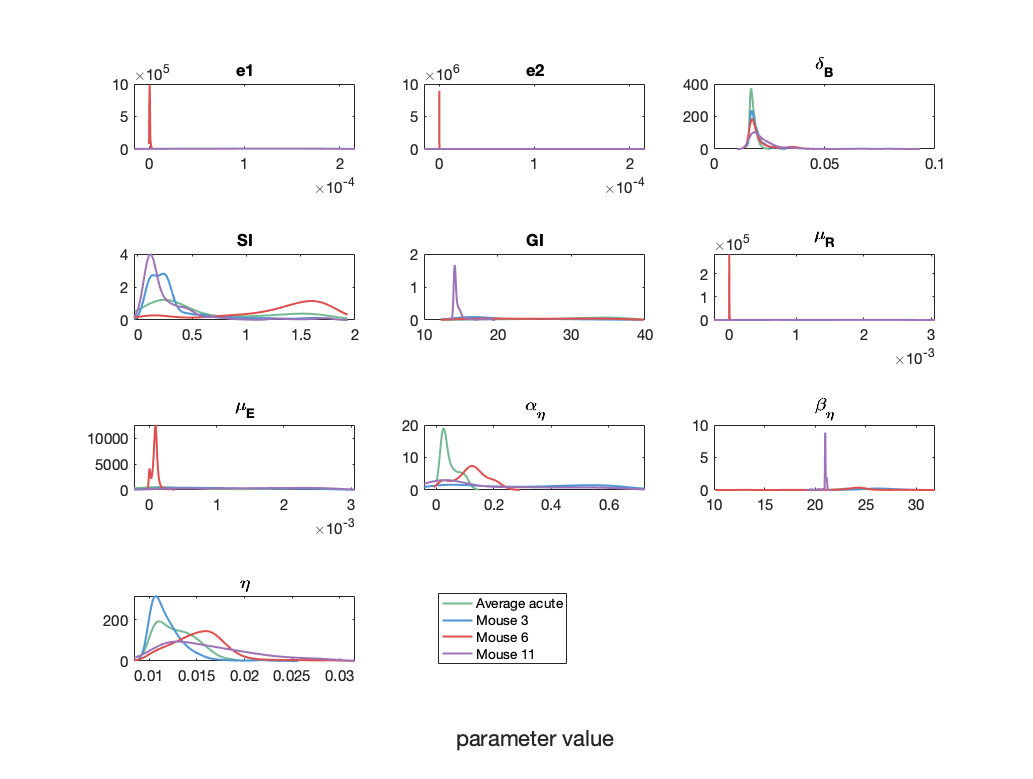
\includegraphics[width=18cm]{MCMC_figs/dram_t1d_final/PDFs_3_6_11_avg.png}
    \caption{Comparison of parameter posterior distributions from DRAM parameterizations performed on Mice 3, 6, 11 data and averaged acute data. Some parameter distributions appear to differ very significantly: e1, e2, GI, $\mu_R$, $\mu_E$, $\beta_eta$. These differences are somewhat expected as we are fitting parameterizations using different data sets. Other parameter distributions appear more similar: $\delta_B$ and $\eta$.}
    \label{fig:overlaiddist_t1d}
\end{figure}
From Figure \ref{fig:overlaiddist_t1d}, we can see that there is quite a lot of variation between distributions of parameters between parameterizations on the different data sets. Notably, for parameters e1, e2, $\mu_R$, and $\mu_E$, the Mouse 6 parameterization have distinctly ``spiked" distributions with significantly greater mean values. The same is true for the Mouse 11 parameterization for parameters GI and $\beta_\eta$. We are unsure of the cause of these thin lone spikes, however we can reason that perhaps the algorithm was unable to sample a larger range for these parameter values. It is interesting to note that parameters e1, e2, $\mu_R$, and $\mu_E$ also have very low Geweke values (Table \ref{tab:6mcmc}). These low convergence diagnostic values in combination with the spiked distribution further indicate that the algorithm appears to have gotten stuck in a small range of values and was likely rejecting a majority of the candidates (and alternatives). We are pleased to see that for parameters $\delta_B$, SI, $\alpha_\eta$, and $\eta$, the distributions between parameterizations are more similar. In particular, the distributions for $\delta_B$ are very similar in shape.
\par Next, we visually compare the resulting glucose predictions below.
\begin{figure}[H]
    \centering
    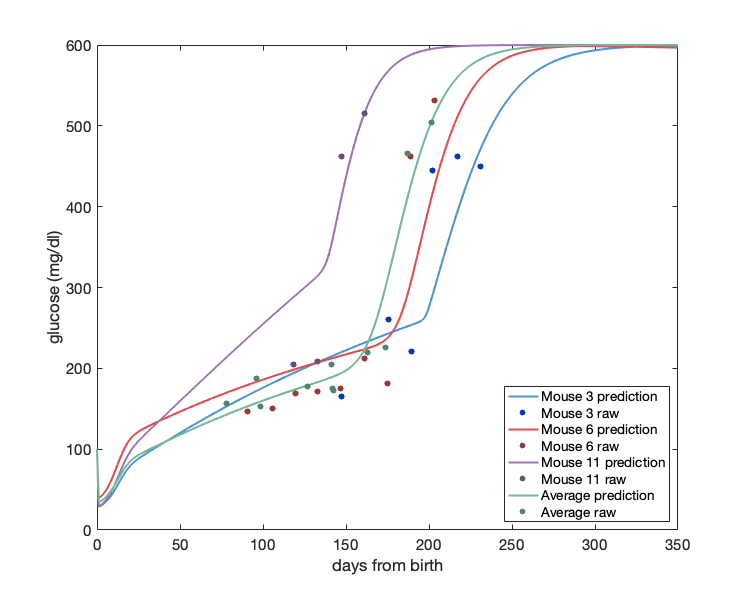
\includegraphics[width=15cm]{MCMC_figs/dram_t1d_final/comp_3_6_11_avg_finalfig.png}
    \caption{Comparing glucose predictions of DRAM parameterizations for mouse 3, mouse 6, mouse 11, and averaged acute data. Through the differences in pivot points and slopes of the starting behaviors, we can see that the data the algorithm begins with is important in determining the final model prediction, particularly in determining the diabetes onset time.}
    \label{fig:21mcmc}
\end{figure}
The overall shapes and behaviors are similar between runs. The largest differences are in the starting behavior slopes and diabetes onset times. We attribute most of these differences to the differences in the original data used during the individual parameterizations. For example, mouse 11's data has the earliest onset time and consequently its prediction has the earliest onset time. The same can be said for mouse 3 which has the latest onset time in both the raw data and prediction. This figures tells us that data seems to play a key role in determining the final model predictions and thus the final parameter values. For a more formal comparison, we calculate the root mean squared error for each prediction using its respective raw data.
\begin{table}[H]
\centering
        \begin{tabular}{c | c}
            \cline{1-2}
            \textbf{Data Set}  &\textbf{RMSE}\\
            \hline
            Mouse 3 & 75.2\\
            Mouse 6 & 66.8\\
            Mouse 11 & 66.3\\
            Average & 30.7
             \\\hline
            \hline
        \end{tabular}
    \caption{Comparison of glucose predictions produced by DRAM using original data from mouse 3, 6, 11 and averaged acute data. RMSE was calculated individually. Based on the RMSE scores, the algorithm captures the averaged data best.}
    \label{tab:7mcmc} 
\end{table}
The RMSE scores tell us that the prediction based on averaged data seems to capture the original data (average acute) the best, although the individual mouse predictions each seem to be performing comparably. While it seems we have a clear best prediction, it is less clear why the averaged data parameterization produced the best results. Perhaps it is because Mice 3 and 11 do not have as many data points. We hypothesize that the number of data points affects the likelihood sum of squares function (recall Step 6d of the DRAM algorithm). Let's say we have 5 data points and we calculate the sum of squares function with a prediction of the ODE model. But we are only able to compare the prediction at these 5 data points and thus, even if the prediction does a poor job of capturing the data (resulting in a large sum of squares), this value might not be as great as if we calculated the sum of squares using the same prediction for 100 data points. Recall from Section \ref{The_Acceptance_Criteria} that a larger sum of squares increases the probability of accepting a specific parameter set candidate. Therefore, with fewer data points, our likelihood function and subsequently our acceptance criterion may not provide an acceptance-rejection threshold that will allow us to find the optimal parameter values.
\par Lastly, we are curious to see how much the final parameter mean values from each run of the algorithm differ. We present the following 3 figures that compare means of mouse 6 and the averaged data parameterization only as these have produced the best results according to Figure \ref{fig:21mcmc} and Table \ref{tab:7mcmc}. Error bars were based on the standard deviations of each parameter mean (these can be found in Tables \ref{tab:5mcmc} and \ref{tab:6mcmc}). We have separated the parameter comparisons because of the difference in magnitude as can be observed on the y-axes. Lastly, we note that we choose not to visually compare the parameters e1, e2, $\mu_R$, $\mu_E$, and $\alpha_\eta$ because their means differed by more than a magnitude of 10. This is due to 1) difficulty in side-by-side comparison and 2) if parameter values differ by such a great magnitude, it is reasonable to say that they are significantly different without plotting their error bars.
\begin{figure}[H]
\begin{subfigure}{.5\textwidth}
    \centering
    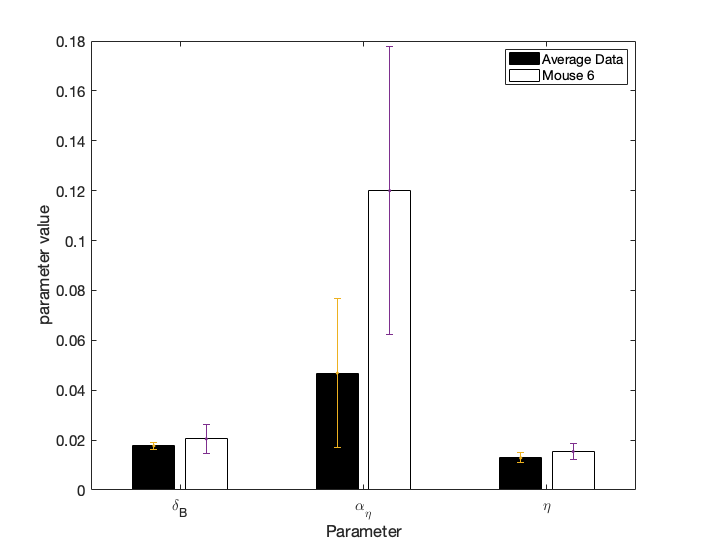
\includegraphics[width=.8\linewidth]{MCMC_figs/dram_t1d_final/mouse6_avg_paramComp1.png}
    \caption{Mean comparison for parameters $\delta_B$, $\alpha_{\eta}$, and $\eta$. Error bars were created using 1 standard deviation in \textbf{Tables \ref{tab:6mcmc} and \ref{tab:5mcmc}}. There does not appear to be a statistical difference between means of these 3 parameters.}
    \label{fig:22mcmc}
\end{subfigure}
\begin{subfigure}{.5\textwidth}
    \centering    
    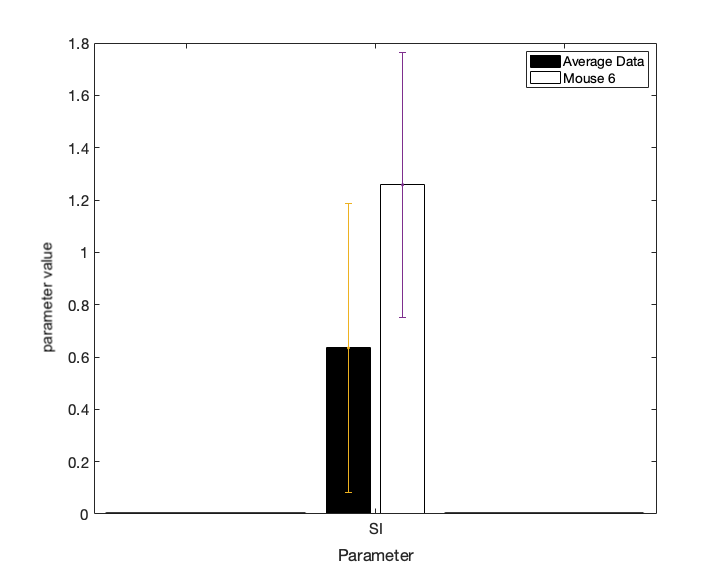
\includegraphics[width=.8\linewidth]{MCMC_figs/dram_t1d_final/mouse6_avg_paramComp_SIONLY.png}
    \caption{Mean comparison for parameters SI. Error bars were created using 1 standard deviation in \textbf{Tables \ref{tab:6mcmc} and \ref{tab:5mcmc}}. There does not appear to be a statistical difference between the means of SI.}
    \label{fig:23mcmc}
\end{subfigure}
\begin{center}
\begin{subfigure}{.5\textwidth}
    \centering
    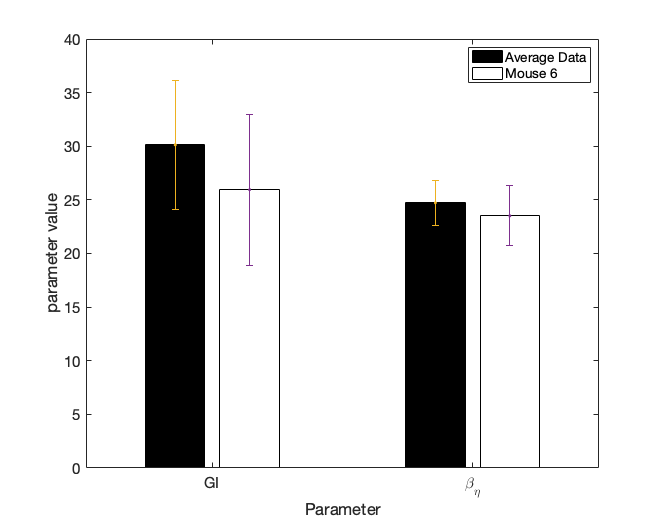
\includegraphics[width=.8\linewidth]{MCMC_figs/dram_t1d_final/mouse6_avg_paramComp2.png}
    \caption{Mean comparison for parameters GI, $\beta_{\eta}$. Error bars were created using 1 standard deviation in \textbf{Tables \ref{tab:6mcmc} and \ref{tab:5mcmc}}. There does not appear to be a statistical difference between the 2 parameters.}
    \label{fig:24mcmc}
\end{subfigure}
\end{center}
\end{figure} 


From these comparisons, we note that 6 out of our our 10 total parameter means are not significantly different between data sets. This gives us some more insight into the differences between convergent parameters in both runs of the algorithms. For example, the 3 common converged parameters between averaged and mouse 6 predictions are $\delta_B$, GI, $\beta_{\eta}$, and $\eta$, these parameters seem to be the most similar in value, therefore we can feel relatively confident in their respective mean values. On the other hand, SI is the only parameter that we have compared (Figure \ref{fig:23mcmc}) that did not converge for either run of the algorithm, we are therefore much more suspicious of these values. 

\paragraph{Takeaways}
Overall, we are satisfied with the DRAM's performance in estimating parameters for the Type 1 diabetes model. We are most impressed with the parameter estimation for the averaged data, as the DRAM seems to perform the best on this data set. As we will discuss in the following sections, we continue to estimate parameters for the T1D model and finally compare the performance of each algorithm.
